\chapter{Implementation}
\label{chap:implementation}

This chapter addresses the implementation of the design detailed before. First, the technical decisions will be presented, followed by a technical view of the software developed. The next section explains how the software was tested by displaying some code examples. Finally, a brief synopsis closes this chapter.

\section{Technical Decisions}
\label{sec:implementation:decisions}

This section describes and justifies the decisions taken while developing \textbf{Sensae Console}.
As a green field project, \textbf{Sensae Console} lacks constraints imposed by prior work. As such, all decisions have been taken during the thesis time span.

The following list unveils the most relevant technical decisions for \textbf{Sensae Console}:

\begin{itemize}
    \item \nameref{subsec:implementation:decisions:backend};
    \item \nameref{subsec:implementation:decisions:frontend};
    \item \nameref{subsec:implementation:decisions:graphql};
    \item \nameref{subsec:implementation:decisions:rabbitmq};
    \item \nameref{subsec:implementation:decisions:proto}
    \item \nameref{subsec:implementation:decisions:database};
    \item \nameref{subsec:implementation:decisions:drools};
    \item \nameref{subsec:implementation:decisions:js};
    \item \nameref{subsec:implementation:decisions:docker};
    \item \nameref{subsec:implementation:decisions:compose};
    \item \nameref{subsec:implementation:decisions:nginx};
    %\item \nameref{subsec:implementation:decisions:git};
    %\item \nameref{subsec:implementation:decisions:issues};
    \item \nameref{subsec:implementation:decisions:actions};
    \item \nameref{subsec:implementation:decisions:maven};
\end{itemize}

\subsection{Backend Technologies Usage throughout the Solution}
\label{subsec:implementation:decisions:backend}

The backend development is divided into three main areas:

\begin{itemize}
    \item \textit{iot-core} package;
    \item Data Flow Scope backend containers;
    \item Service and Configuration Scope backend containers (named \nameref{subsubsec:implementation:decisions:backend:geral});
\end{itemize}

In the following sub sections a brief description and justification of the technologies used is presented.

\subsubsection{Programming Language Used}
\label{subsubsec:implementation:decisions:backend:prog}

A package named \textit{iot-core}, an idealized \gls{SDK} for \textbf{Sensae Console}, was developed to define the information that flows inside the system.
The \textit{iot-core} package was developed in \textit{Java}.

In the future, more programming languages may be supported though new \gls{SDK}s. The \textit{Rust} programming language is the next candidate due to its low memory footprint, fast startup times and expressive syntax.

The reasons that lead to the development of it in \textit{Java} are:

\begin{itemize}
    \item It's the programming language that the author is most familiarized with;
    \item It is widely used in industry for backend service development;
    \item Vast and robust support for virtually any technology used for backend development: database access, synchronous and asynchronous communication protocols, streaming platforms, embedded caches, rule engines and script engines.
\end{itemize}

The development of \textit{iot-core} in \textit{Java} lead to the development of all backend services also in \textit{Java}.

\subsubsection{General Backend Services}
\label{subsubsec:implementation:decisions:backend:geral}

The services that this section encompasses can be seen as more robust and heavy due to their associated requirements.

As such, the framework used to develop them was \citetitle{springboot}, due to its vast documentation and big community. This framework comes with several modules that help to easily create stand-alone, production-grade applications. The author also had previously worked with this framework.

The main drawbacks of this framework are the slow start up time and high memory consumption, since these are not ideal for the microservices/cloud world [\cite{springslow}].

\subsubsection{Data Flow Scope Backend Services}
\label{subsubsec:implementation:decisions:backend:flow}

As discussed in Section~\ref{subsec:design:system_scopes:data_flow_scope}, the services that this section encompasses can be seen as more lightweight than the ones described above due to their associated requirements.

Since this containers process inbound device data, they have a bigger need to automatically scale. Since they need to react faster to throughput changes, their start up times must be small.

As such, the framework used to develop them was \citetitle{quarkus}. This framework has first-class support for \citetitle{graalvm}.

According to \cite{graalvm-intro}, GraalVM is a ``high-performance JDK designed to accelerate the execution of applications written in Java and other JVM languages while also providing runtimes for JavaScript, Python, and a number of other popular languages. GraalVM offers two ways to run Java applications: on the HotSpot JVM with Graal just-in-time (JIT) compiler or as an ahead-of-time (AOT) compiled native executable. GraalVM's polyglot capabilities make it possible to mix multiple programming languages in a single application while eliminating foreign language call costs.''

This features, coupled with the fact that the \textit{Quarkus} architecture follows the \citetitle{reactivemanifesto}, are appealing when compared with \citetitle{springboot} that only has experimental support for \citetitle{graalvm}, via \citetitle{spring-native}.

\subsection{Frontend Technologies Usage through the Solution}
\label{subsec:implementation:decisions:frontend}

Even though a micro frontend architecture empowers the selection of different technologies depending on the requirements of the solution and team affinity with the stack, the Frontend Containers were developed using the same technological stack. At the time of writing there was only one developer involved, this diminished the cognitive load needed to work on the solution while still allowing future collaborators to use different frontend frameworks.

\subsubsection{Programming Language and Framework Used}
\label{subsubsec:implementation:decisions:frontend:prog}

The author had previous contact with the following frameworks: (i) \citetitle{angular}, (ii) \citetitle{react}, and therefore no other tool was discussed when choosing the one to use in the solution.

The programming language used was \citetitle{typescript} since it is a strongly typed language and therefore leads to more robust and predictable code. Static typing helps to avoid various bugs that arise when using \citetitle{javascript}. Before transpiling \citetitle{typescript} code to \citetitle{javascript}, it is analyzed to detect bugs related to type errors.

As for the framework/library used, the following table, Table~\ref{tab:implementation:decisions:frontend:prog}, describes the reason that lead the author to choose Angular over React.

\begin{table}[H]
    \caption{Technologies Comparison - Angular vs React}
    \label{tab:implementation:decisions:frontend:prog}
    \centering
    \begin{tabular}{@{}cll@{}}
    \toprule
    \textbf{Framework/Library}                                                                 & \textbf{Angular} & \textbf{React}           \\ \midrule
    \begin{tabular}[c]{@{}c@{}}Separation of User Interface\\  and Business Logic\end{tabular} & enforced         & flexible                 \\ \midrule
    Language Requirements                                                                      & typescript       & javascript or typescript \\ \midrule
    Familiarity with the tool                                                                  & high             & medium                   \\ \midrule
    \begin{tabular}[c]{@{}c@{}}UI Component Libraries with wide\\  community support\end{tabular} &
      material &
      \begin{tabular}[c]{@{}l@{}}ant design, material ui, \\ react bootstrap, semantic ui react\end{tabular} \\ \bottomrule
    \end{tabular}
\end{table}

Both tools have a wide support from the community and excellent documentation. For the author, Angular outclasses React in this project since it enforces the use of good design principles via the first and second entry described in Table~\ref{tab:implementation:decisions:frontend:prog}.

\subsubsection{Technologies used to create a Micro Frontend Architecture}
\label{subsubsec:implementation:decisions:frontend:micro}

\citetitle{modulefederation} was the tool used to seemly connect the various Frontend. No other tool was considered or researched since \textit{Angular} already relies on \textit{Webpack 5} to bundle the application and therefore it's effortless to use this tool. \citetitle{modulefederation} allows programs to reference other programs parts that are not known at compile time. In addition, the micro frontends can share libraries with each other, so that the individual bundles do not contain any duplicates.

\subsubsection{Technologies used to build and manage the Frontend Services}
\label{subsubsec:implementation:decisions:frontend:nx}

This section describes how the various frontends are built and share common pieces of code. Angular comes with a tool to build and manage project but it was deemed too minimal for this project. Instead, the tool used was \citetitle{nx}. \citetitle{nx} describes it self as a ``Smart, Fast and Extensible Build System'', the
``Next generation build system with first class monorepo support and powerful integrations.''

This tool provides features needed to manage multiple frontends in a single repository, without dealing with libraries versions mismatch.

This tool has two main concepts that are widely used in the solution's frontend: apps and libraries. Apps focus on the \gls{UI} and libraries on everything else, such as the domain or the interactions with backend services. The diagram presented before at Figure~\ref{fig:design:architecture:platform:component:development:diagram:decoder} resembles this two concepts.

\subsubsection{Technologies used to provide map/location base services}
\label{subsubsec:implementation:decisions:frontend:maps}

This section briefly describes the library used to render and work with maps.

The two options in regards to this requirement were: (i) \citetitle{googlemaps} and (ii) \citetitle{mapbox}.

The author picked \citetitle{mapbox} due to better documentation, a more stable \gls{API}, and a much suitable pricing plan for small businesses, when compared to \citetitle{googlemaps}.

This library can render custom maps and is bundled with powerful data visualization tools with a simple to use \gls{API}, two features deemed important for the solution.

\subsection{Backend Services Expose a GraphQL API}
\label{subsec:implementation:decisions:graphql}

The \gls{API} discussed in this section refers to the interfaces exposed to the outside world by backend containers of the Configuration and External Services Scopes and isn't related to the internal communication or device data ingestion interface exposed by the \textbf{Data Relayer} Container.

The two approaches considered were: (i) \citetitle{rest} and (ii) \citetitle{graphql}.

According to \cite{graphql}, ``GraphQL provides a complete and understandable description of the data in your API, gives clients the power to ask for exactly what they need and nothing more, makes it easier to evolve APIs over time, and enables powerful developer tools.''

According to \cite{rest}, ``REST APIs provide a flexible, lightweight way to integrate applications, and have emerged as the most common method for connecting components in microservices architectures.''

These two approaches have vast differences but they both try to answer the same question: How should one expose internal data to the outside world?

\cite{eizinger2017api}, compares these two approaches under five criteria: (i) operation reusability, (ii) discoverability, (iii) component responsibility, (iv) simplicity, (v) performance, (vi) interaction visibility and (vii) customizability.

\citetitle{graphql} was the chosen approach mainly due to better operation reusability: ``The flexibility in the definition of the exactly returned data allows clients to tailor it for their specific needs, thereby achieving highly reusable data retrieval operations.'' and interaction visibility: ``With GraphQL featuring a declarative language, intermediaries capable of understanding the GraphQL grammar can at least partly reason about the communication between a client and a GraphQL server.''

\cite{eizinger2017api}, when discussing the complexity of each approaches also highlights that ``GraphQL makes fetching data in various ways really simple for the client.''

The idea behind the highly decoupled architecture of this solution derives from the need to provide knowledgeable customers with the tools to easily design and incorporate their solutions in \textbf{Sensae Console}. The usage of \citetitle{graphql} further complements this idea by providing an API that is simple to understand and consume.

\subsection{Usage of RabbitMQ to support Internal Communication}
\label{subsec:implementation:decisions:rabbitmq}

As discussed in Section~\ref{subsec:design:alternatives:flow} and \ref{subsec:design:alternatives:internal}, the technology needed for this solution had to act as a message broker. It should enable the system to follow a push approach and ease the complex routing model envisioned.

The technology chosen for internal communication was \citetitle{rabbitmq}. This message broker was chosen in detriment of others since the author had previously worked with the technology and, according to \cite{10.1145/3093742.3093908} ``RabbitMQ would be a good choice for realtime processing, based on the complex filtering the broker could provide''.

\cite{10.1145/3093742.3093908} also mentions that RabbitMQ would be best-suited to be the Underlying Layer for IoT Applications Platform.

The exchange that better fits the defined requirements is the Topic Exchange, due to the possibility to subscribe to specific messages depending on their routing keys (as mentioned in Section~\ref{par:stateofart:arch:infra:mediator:rabbitmq}).

When working with this protocol and type of exchange, some drawbacks were found:

When dealing with Topic Exchanges a Consumer can only subscribe to one specific routing key or all at once - via \textit{*}- this makes it complex to create routing keys with dynamic values. As an example, lets look at the \textit{Channel} routing key defined in Table~\ref{tab:design:domain:shared_model:routing} of Section~\ref{subsubsec:design:domain:shared_model:routing}. This key defines the single destination of a data unit. For a data unit to have various dynamic service destinations there would be a need to either:

\begin{itemize}
    \item Ensure that every single service subscribes to all relevant combinations of \textit{channel}s possible, deemed impractical;
    \item Duplicate data units, where each copy would be assigned a different channel, deemed inefficient;
\end{itemize}

To tackle this issue, another Message Broker, such as \citetitle{pulsar}, with its own protocol, can be used in the future. This Message Broker answers the drawback describe above by allowing Consumers to subscribe to multiple topics (equivalent to RabbitMQ' routing keys) on the basis of a regular expression (regex) [\citetitle{pulsarmulti}].

The other drawback found is that, according to the \citetitle{rabbitmqprotocol} the routing keys have a max size of 255 bytes. As described in Table~\ref{tab:design:domain:shared_model:routing} of Section~\ref{subsubsec:design:domain:shared_model:routing}, the system currently supports various keys and more keys are expected to be added in the future, meaning that this cap may one day be reached. This limitation was tackled by mapping each routing key to a single character when possible. As an example, the routing key \textit{Info Type Options} in Table~\ref{tab:design:domain:shared_model:routing} has three possible values: Encoded, Decoded and Processed, theses values are respectively represented in the system as \textit{e}, \textit{d} and \textit{p}.

\subsection{Usage of Protocol Buffers in Internal Communication}
\label{subsec:implementation:decisions:proto}

This section refers to how messages that flow in the system (via Message Broker) are serialized and deserialized. The common formats used to send structured data across systems are \gls{JSON} and \gls{XML}. This formats sacrifice size and de/serialization performance for human readability as stated by \cite{sumaray2012comparison}.

As mentioned before, \textbf{Sensae Console} aims to provide a good developer experience for external costumers that want to expand the solution according to their needs. Due to this, the final decision weighted heavily on formats that were self-documented, e.g. defined by a strict \textit{data schema}, such as \citetitle{proto} and \citetitle{thrift}.

These two technologies, \citetitle{proto} and \citetitle{thrift}, have similar goals and approaches to the problem they try to solve. They both rely on code generation based on a schema of the data structure. The tools related to this formats officially support various languages such as \textit{Java}, \textit{C++}, \textit{C\#}, \textit{Python}, \textit{Go} and others.

By leveraging these features, creating a basic \gls{SDK} in a new programming language is trivial since serialization, deserialization and data structure is already taken care by the code generation tool.

\citetitle{proto} are a ``language-neutral, platform-neutral, extensible mechanism for serializing structured data'' [\cite{proto}].

Thrift's ``primary goal is to enable efficient and reliable communication across programming languages by abstracting the portions of each language that tend to require the most customization into a common library that is implemented in each language'' [\cite{thrift}].

Ultimately \citetitle{proto} were chosen due to better documentation and community support.

\subsection{Database Usage throughout the Solution}
\label{subsec:implementation:decisions:database}

This section refers to how information is stored across the system and follows the terms mentioned in Section~\ref{subsubsec:stateofart:arch:infra:store}.

The requirements gathered unveil the need to use three different database data models throughout the system: (i) relational, (ii) document-based and (iii) column-based data models. The following sections answer why these data models were needed and what technologies were chosen for each of them. A final section unveils an optional solution that was considered but ultimately not pursued.

\subsubsection{Relational Database Usage}
\label{subsubsec:implementation:decisions:database:relational}

This type of data, strict and with well-defined relations, can be found on most Bounded Concerns described in Section~\ref{subsec:design:domain:bounded_contexts} such as \nameref{subsubsec:design:domain:bounded_contexts:processor}, \nameref{subsubsec:design:domain:bounded_contexts:decoder}, \nameref{subsubsec:design:domain:bounded_contexts:device}, \nameref{subsubsec:design:domain:bounded_contexts:identity}, \nameref{subsubsec:design:domain:bounded_contexts:rule} and the Irrigation Zone/Device concepts of the \nameref{subsubsec:design:domain:bounded_contexts:irrigation} Concern.

As such, this data model was adopted for the \textbf{Device Management Database}, \textbf{Data Decoder Database}, \textbf{Data Processor Database}, \textbf{Rule Management Database}, \textbf{Identity Management Database}, \textbf{Smart Irrigation Business Database} and \textbf{Notification Management Database} containers. The decision was based on the discussion in Section~\ref{par:stateofart:arch:infra:store:relational}.

The decision to use \citetitle{postgressql} was taken based on the fact that, contrary to the other options, \citetitle{postgressql} supports a vast number of Data Types such as \gls{JSON}, Arrays, \gls{UUID}, and Ranges. \citetitle{postgressql}'s data model is an extension of the relation data model, named object-relational data model - \cite{elmasri2000fundamentals}. This data model supports various concepts such as objects, classes and inheritance and therefore can lead to entity models more expressive and close to the business ideas.

\subsubsection{Document-based Database Usage}
\label{subsubsec:implementation:decisions:database:nosql}

The type of features of this data model resembles the requirements and data stored by the Data Store container described in Section~\ref{subsec:design:system_scopes:data_flow_scope} and Figure~\ref{fig:design:architecture:platform:container:process:diagram:flow}. This container, intended to mimic a Data Lake\footnote{Massively scalable storage repository that holds a vast amount of raw data in its native format («as is») until it is needed, by \cite{miloslavskaya2016big}}, stores any type of data for future use.

As such, this data model was adopted for the \textbf{Data Store Database} container. The decision was based on the discussion in Section~\ref{par:stateofart:arch:infra:store:nosql}.

The only technology considered, and therefore adopted, was \citetitle{mongodb} due to its vast community, excellent documentation, open-source license and large number of libraries that ease the database management operations. \citetitle{mongodb} also supports replication and sharding. According to \cite{elmasri2000fundamentals}, these features are useful once a single node isn't capable of withstanding all data collected while providing fast access to it.

\subsubsection{Column-based Database Usage}
\label{subsubsec:implementation:decisions:database:time}

The features mentioned in Section~\ref{par:stateofart:arch:infra:store:time} fit the requirements related to storing and reading vast amounts of device measures. As such, this database type was adopted for the \textbf{Fleet Management Database} and \textbf{Smart Irrigation Data Database} containers.

The type of business this solution tackles revolves around the capture and analysis of device readings. So the notion of time has to be treated as a first class citizen. The measurements that constitute a time series are ordered on a timeline, which reveals information about underlying patterns.

As stated by \cite{naqvi2017time}, \gls{TSDB} ``can be used to efficiently store sensors and devices' data'' since, ``such technologies are generating large amount of data which is usually time-stamped''.

With this requirements in hand, a column-based data model isn't enough. The technology adopted should also natively support time series to ease data analysis. As such, the \citetitle{hbase} and \citetitle{cassandradb} options were discarded.

Between the two missing options, the author picked \citetitle{questdb} due to better support for \gls{SQL} though \gls{JDBC}. During the research of this two technologies no major downside was found for \citetitle{questdb} when compared to \citetitle{influxdb}.

The author had no previous contact with this type of data model.

\subsubsection{Graph-based Database Usage}
\label{subsubsec:implementation:decisions:database:identity}

Even tho this data model was ultimately not used, the author deemed relevant to analyze it.

As stated in the bounded context's section of~\nameref{subsubsec:design:domain:bounded_contexts:identity}, the domains follow a hierarchical structure that can resemble a graph. This context in particular would benefit from a  graph-based database, but this option was not pursued since the author had no previous contact with this family of technologies. Instead \citetitle{postgressql} was used.

\citetitle{postgressql} can represent logical hierarchical structures and concepts using the array data type as the \textit{path} from the root domain to the current domain.

Queries that revolve around graph concepts such as: select parent node, select child nodes, move nodes to a new parent and others, can be preformed efficiently using array operators such as \textbf{\&\&}, \textbf{||} and \textbf{@>}\footnote{taken from PostgresSQL Documentation: \citetitle{postgresarray} \& \citetitle{postgresarrayop}}.

\subsection{Rules Script Engine}
\label{subsec:implementation:decisions:drools}

This section refers to the bounded context of \textbf{Rule Management}. As mentioned before, the purpose of this context is to provide a high-level language that can analyze a stream of Data Units and output alerts base on them. The technology adopted was \citetitle{drools}.

\citetitle{drools} is a rule engine widely used in the industry \parencite{droolsindustry}. The features that stud out from other rule engines mentioned in \ref{subsubsec:stateofart:arch:infra:rule}:

\begin{itemize}
    \item Open-source license;
    \item Support for sliding windows of time;
    \item It is also a \gls{CEP} System;
    \item Integrates with the \textit{iot-core} package since it is also written in \textit{Java};
    \item Can be used as a standalone application or an embedded component of another application;
    \item Has an expressive, yet complex, syntax to write rules;
    \item Can dynamically load rules at runtime.
\end{itemize}

The Section~\ref{subsec:implementation:description:rule} details how one can write rule scenarios.

\subsection{Data Decoders Script Engine}
\label{subsec:implementation:decisions:js}

This section refers to the bounded context of \textbf{Data Decoder}. As mentioned before, this context purpose is to translate inbound Data Units into a format and semantics that the system can understand. The technology adopted was \textit{Javascript}.

\textit{Javascript} is a high level language with an enormous community and is widely used in the industry. Another big reason behind this decision is that a lot of companies producing \gls{IoT} devices provide open-source decoders written in \textit{Javascript}, such as \href{https://github.com/Milesight-IoT/SensorDecoders}{Milesight} \footnote{\href {https://github.com/Milesight-IoT/SensorDecoders}{github.com/Milesight-IoT/SensorDecoders}}, \href{https://github.com/SensationalSystems}{SensationalSystems} \footnote{\href {https://github.com/SensationalSystems}{github.com/SensationalSystems}} and \href{https://github.com/helium/console-decoders}{Helium}, \footnote{\href {https://github.com/helium/console-decoders}{github.com/helium/console-decoders}}. This makes it easy and straightforward to integrate new decoders in \textbf{Sensae Console}.

The Section~\ref{subsec:implementation:description:decoder} details how one can write decoders.

\subsection{Containerization of services via Docker}
\label{subsec:implementation:decisions:docker}

This section describes how the final product is packaged into containers.

As stated in \citetitleyear{dockerinit}, Docker acts as an intermediary layer between the application to be deployed and the operating system where it will be deployed, ensuring that the developed software has the same behavior regardless of the system. The dependencies of the solution do not have to be present in the system, it is only necessary to install the Docker tool in the \gls{OS}.

This tool thus makes it possible to lower the coupling between the \gls{OS} and the software to be deployed.

With regards for this solution, each container defined in Section~\ref{sec:design:architecture} is mapped into a docker container.
A container is often compared to a virtual machine running on a hypervisor or \gls{OS}, but it has a much lower resource consumption, since only the application runs and not not all the processes inherent to an \gls{OS} as described by \cite{bernstein2014containers}.

The Figure~\ref{fig:implementation:decisions:docker:contvsvm} compares a \gls{VM} and Container-based deployments.

\begin{figure}[H]
    \centering
    \resizebox{0.7\columnwidth}{!}
    {
       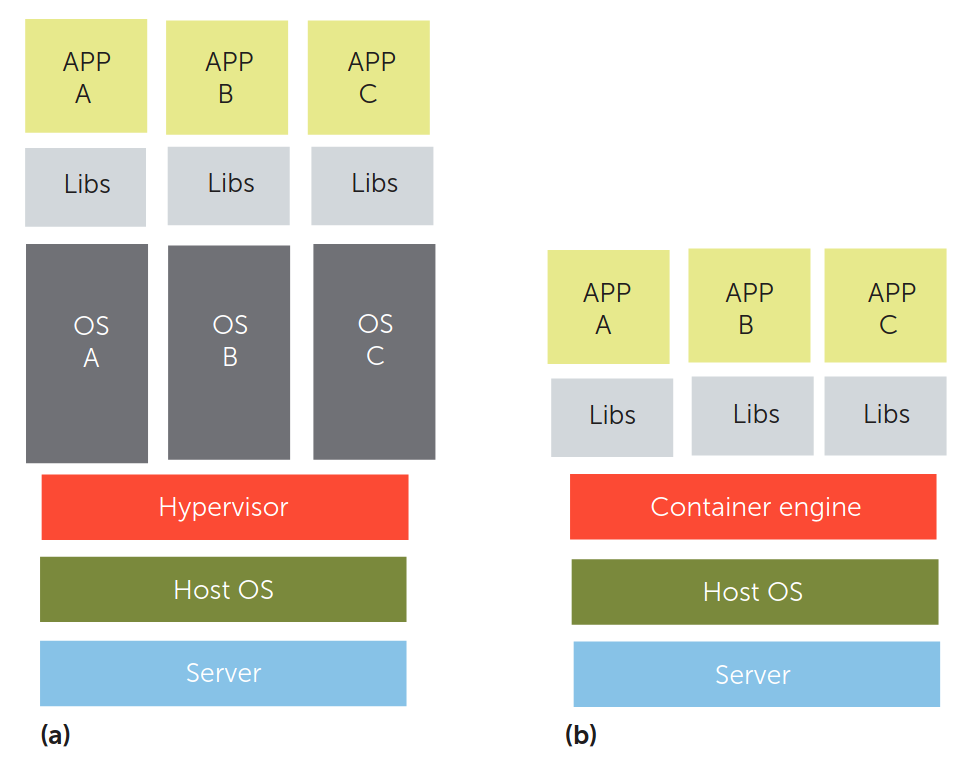
\includegraphics{assets/figures/vmvscontainer.png}
    }
    \caption[Comparison of VM and Container-based deployments]{Comparison of VM (a) and Container-based (b) deployments by \cite{bernstein2014containers}}
    \label{fig:implementation:decisions:docker:contvsvm}
\end{figure}

The system is thus represented as a collection of containers that communicate with each other and the outside through standard protocols such as HTTP or \gls{AMQP}.

The production environment can thus be quickly replicated on another machine in case of a failure disaster or a overwhelming number of interaction with the server.

Details about service containerization can be found in Section~\ref{subsec:implementation:description:docker}.

\subsection{Orchestration of services via Docker Compose}
\label{subsec:implementation:decisions:compose}

This section describes how the final product is orchestrated using Docker Compose.

As stated in the article \citetitleyear{dockercompose}, ``Compose is a tool for defining and running multi-container Docker applications''.

Currently a single node is capable of handling the traffic generated by all the managed devices and costumers. Due to this, it was decided to use a docker compose in production inserted of tools like Kubernetes (that can ease the process of autoscaling individual containers).

The solution's orchestration is defined in a \textit{YAML} file and then started with a single command. To improve security, only the needed container ports are exposed. To ensure data integrity throughout service disruptions, persistence data is mapped to folder in the \gls{OS}. To ensure an easy management of the environment, configurations are kept in the \gls{OS} and fetched by each container once they start.

The details about the solution orchestration can be found in Section~\ref{subsec:implementation:description:compose}.

\subsection{Usage of Nginx as a web server and reverse proxy}
\label{subsec:implementation:decisions:nginx}

To serve the frontend pages and redirect requests made to backend containers, the following technologies were analyzed:

\begin{itemize}
    \item \citetitle{nginx};
    \item \citetitle{apachehttp};
    \item \citetitle{lighttpd}.
\end{itemize}

All of them support the necessary requirements, but some factors lead the author to pick Nginx over the others, the following table, Table~\ref{tab:implementation:decisions:nginx:compare}, describes this criteria.

\begin{table}[H]
    \caption{Technologies Comparison - Reverse Proxy Web Server}
    \label{tab:implementation:decisions:nginx:compare}
    \centering
    \begin{tabular}{@{}clll@{}}
    \toprule
    \textbf{Criteria/Technology} & \textbf{Nginx} & \textbf{Apache HTTP Server} & \textbf{Lighttpd} \\ \midrule
    Resource Consumption      & low  & high      & medium \\ \midrule
    Community Size            & high & very high & medium \\ \midrule
    Familiarity with the tool & high & low       & low    \\ \bottomrule
    \end{tabular}
\end{table}

The details about \citetitle{nginx} adoption and configuration can be found in Section~\ref{subsec:implementation:description:nginx}.

% \subsection{Usage of Git as a version control system of the project}
% \label{subsec:implementation:decisions:git}

% \citetitle{git} is a \gls{VCS}. What differentiates it from other
% systems such as \citetitle{mercurial} and \citetitle{bitkeeper} is its branching model. It is currently also the most widely used.

% \citetitle{github} was the platform used to host the developed code. It offers private repositories with no additional costs. This platform also has other tools such as \textit{Github Issues} and \textit{Github Actions} that ease a developer's workflow.

% A \gls{VCS} is indispensable in software development, this system allows developers to store the history of changes made to the code in an organized manner and simplifies the management of the software by the development team. This system was chosen over others because of the author was experienced with this software.

% The development of the entire solution was made in two separated repositories, one for \textit{iot-core} and another for \textbf{Sensae Console}.

% The \textit{iot-core} repository had a simple branching model consisting only of a master branch.

% There was an extensive use of the branching feature in the repository of \textbf{Sensae Console}, following the model shown in Figure~\ref{fig:implementation:decisions:git:branch}. The author settled for the following: a master branch that matches the deployed version, a development branch where the various features are introduced until a new version is published on the master branch, several branches dedicated to fixing bugs (hotfix) and another several branches that introduce new features and improvements (feature \textit{x}).

% \begin{figure}[H]
%     \centering
%     \resizebox{\columnwidth}{!}
%     {
%        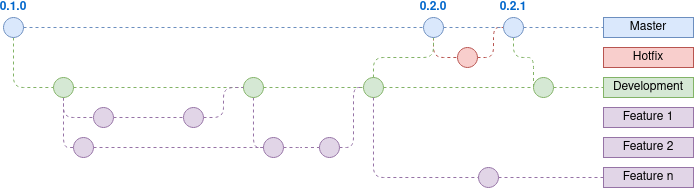
\includegraphics{assets/figures/branching-model.png}
%     }
%     \caption[Branching Model]{Branching Model}
%     \label{fig:implementation:decisions:git:branch}
% \end{figure}

% This model was adopted since the project was in an initial phase of development, in the future, a branching model with multiple releases, as detailed in Figure~\ref{fig:implementation:decisions:git:branch2}, is preferred. With this model one can release only the altered containers and not the entire system.

% \begin{figure}[H]
%     \centering
%     \resizebox{\columnwidth}{!}
%     {
%        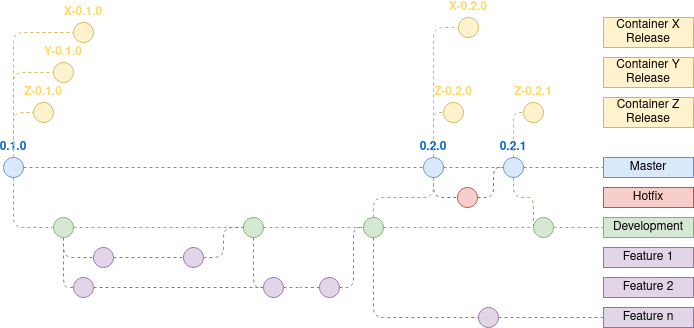
\includegraphics{assets/figures/branching-model-2.png}
%     }
%     \caption[Future Branching Model]{Future Branching Model}
%     \label{fig:implementation:decisions:git:branch2}
% \end{figure}

% This is useful when using CI/CD pipelines to compile, package and deploy the various containers of the solution. If no changes have been made to \textit{X} Container there is no need to redo all the work previously done with it.

% The reason behind the monorepo approach for \textbf{Sensae Console} is that it allows frontend libraries to be shared without publishing somewhere. It is also much easier to keep track of the code in a monorepo since the solution is developed by a single developer.

% \subsection{Usage of Github Issues to track issues, bugs and new features}
% \label{subsec:implementation:decisions:issues}

% As described before, the code is hosted in \citetitle{github}. One of the services that this platform offers is \textit{Github Issues}. This tool helps to track and document the development process alongside with the code.

% This tool can be separated into two main views. A view is concerned about what issues, features and bugs are active in the project, Figure~\ref{fig:implementation:decisions:issues:board}, and the other is concerned with the current state of each issue, feature and bug, Figure~\ref{fig:implementation:decisions:issues:project}.

% \begin{figure}[H]
%     \centering
%     \resizebox{\columnwidth}{!}
%     {
%        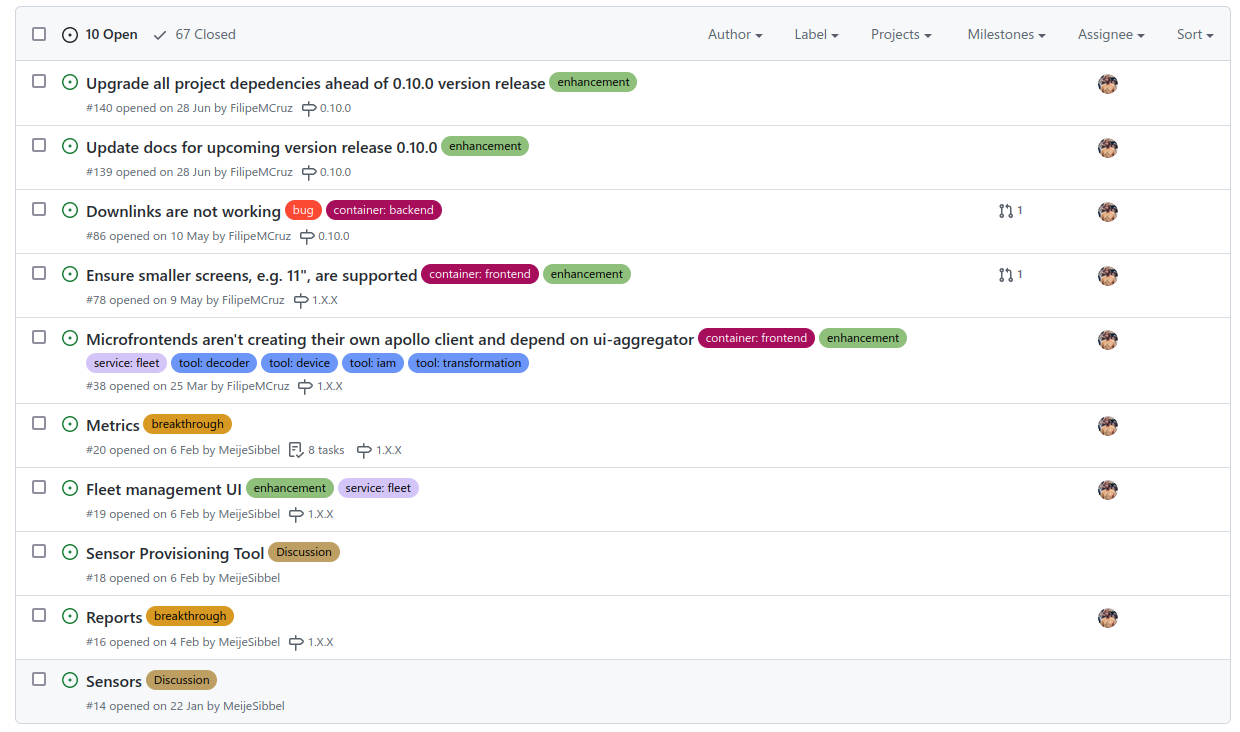
\includegraphics{assets/figures/github-2.png}
%     }
%     \caption[Github Issues]{Github Issues}
%     \label{fig:implementation:decisions:issues:board}
% \end{figure}

% Each issue has a list of tags that represent its scope and a defined milestone. With this tool, the team members can also discuss issues in depth.

% The issues presented in this page are then tracked in the \textit{project} page - Figure~\ref{fig:implementation:decisions:issues:project}. The author decided to divided the issues into 4 criteria:

% \begin{itemize}
%     \item \textbf{To Do}: Issues that have been discussed and are to be completed in the near future;
%     \item \textbf{In Progress}: Issues that are currently under development and have an assigned feature branches;
%     \item \textbf{Done}: Issues that have been completed and have been integrated in the \textit{master} branch;
%     \item \textbf{Future}: Issues that have been purposed but have no clear deadline.
% \end{itemize}

% \begin{figure}[H]
%     \centering
%     \resizebox{\columnwidth}{!}
%     {
%        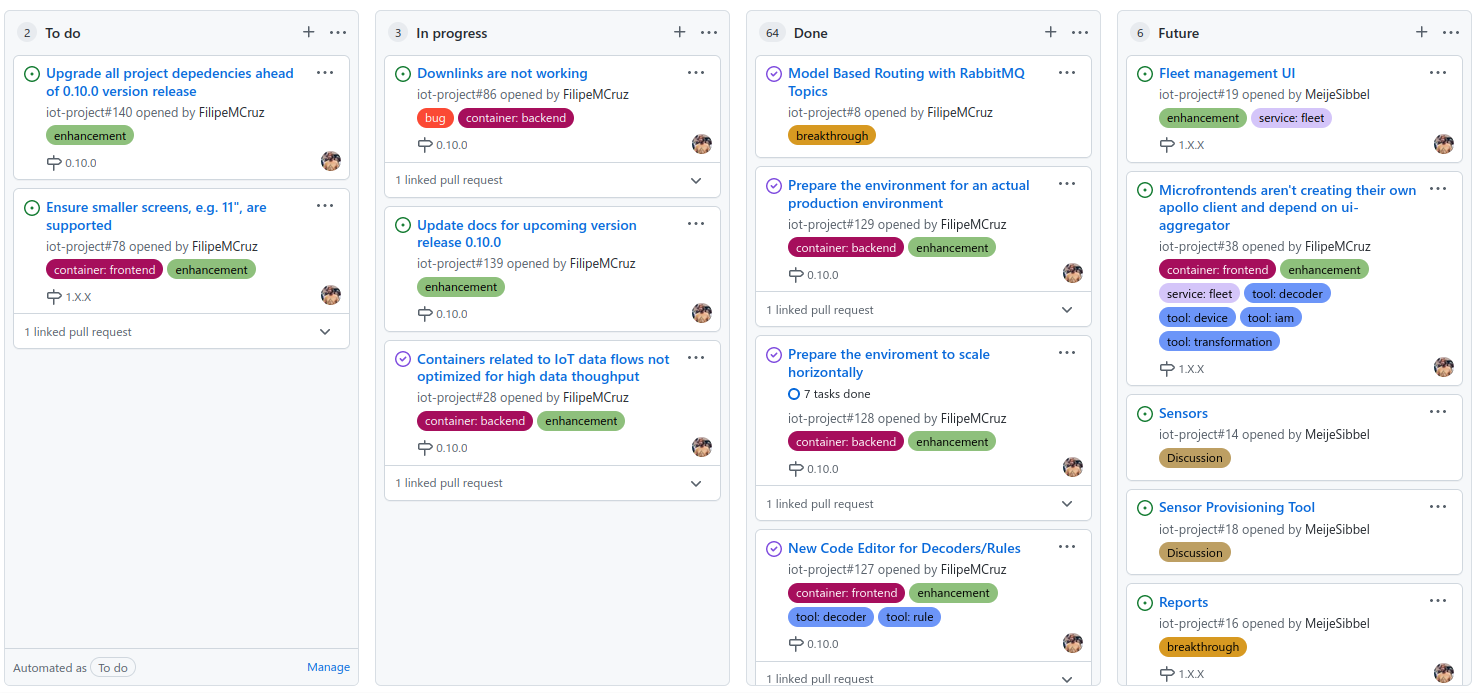
\includegraphics{assets/figures/github.png}
%     }
%     \caption[Github Issues Project Board]{Github Issues Project Board}
%     \label{fig:implementation:decisions:issues:project}
% \end{figure}

% This view helps to define a simple project roadmap and track the overall state of issues, bugs and features in the project.

\subsection{Usage of Github Actions for CI/CD}
\label{subsec:implementation:decisions:actions}

Since the code is hosted in \textit{Github}, it was decided to leverage the CI/CD features of the platform. \textit{Github Actions} purpose is to automate software workflows via CI/CD.

According to \cite{cicd}, the term CI/CD represents a method to delivering applications to clients by introducing automation into the development states.
It is divided into three concepts:

\begin{itemize}
    \item \textbf{Continuous Integration}: new versions of the project are regularly submitted, tested and merged into the current project;
    \item \textbf{Continuous Delivery}: new versions of the project are automatically archived in a repository where they can then be deployed to a production environment;
    \item \textbf{Continuous Deployment}: new versions of the project are automatically deployed to a production environment.
\end{itemize}

The \textit{iot-core} package is archived in a repository so that it can then be integrated in the backend containers of \textbf{Sensae Console}, and possibly in other projects. To do so, the team uses \textit{Github Actions}. This tool's behavior is defined in a YAML file, presented in the Code Sample~\ref{code:implementation:decisions:actions:iotcore}.

\begin{lstlisting}[style=yaml, caption=Configuration File for \textit{iot-core} Continuous Delivery, label={code:implementation:decisions:actions:iotcore}]
name: IoT Core - Continuous Delivery to maven central
on:
  push:
    tags:
      - '**'
      - '*'
jobs:
  build:
    runs-on: ubuntu-latest
    steps:
      - uses: actions/checkout@v2
      - name: Set up Maven Central Repository
        uses: actions/setup-java@v1
        with:
          java-version: 17
          server-id: ossrh
          server-username: MAVEN_USERNAME
          server-password: MAVEN_PASSWORD
          gpg-private-key: ${{ secrets.MAVEN_GPG_PRIVATE_KEY }}
          gpg-passphrase: MAVEN_GPG_PASSPHRASE
      - name: Deploy with Maven
        run: mvn -B clean deploy -Pci-cd
        env:
          MAVEN_USERNAME: ${{ secrets.OSSRH_USERNAME }}
          MAVEN_PASSWORD: ${{ secrets.OSSRH_TOKEN }}
          MAVEN_GPG_PASSPHRASE: ${{ secrets.MAVEN_GPG_PASSPHRASE }}
\end{lstlisting}

As we can see in lines \textbf{2} to \textbf{6}, this action is triggered every time a new git tag is pushed to the repository.
This action then proceeds to download and setup java and maven - lines \textbf{12} to \textbf{20}. Finally it runs a maven command to deploy the new version to the artifact repository - lines \textbf{21} to \textbf{26}.

The \textbf{Sensae Console} has an action to deal with Continuous Integration - Code Sample~\ref{code:implementation:decisions:actions:cisensae}, where changes made to the software are tested.

\begin{lstlisting}[style=yaml, caption=Configuration File for \textbf{Sensae Console} Continuous Integration, label={code:implementation:decisions:actions:cisensae}]
name: Sensae Console - Continuous Integration - Test changes
on:
  push:
    branches:
      - master
      - dev
jobs:
  test:
    runs-on: ubuntu-latest
    steps:
      - uses: actions/checkout@v3
      - name: Set up JDK 17
        uses: actions/setup-java@v3
        with:
          java-version: "17"
          distribution: "adopt"
      - name: Set up Node 16
        uses: actions/setup-node@v3
        with:
          node-version: 16
      - name: Test Suite
        run: |
          ./project/scripts/run-tests.sh "${{ secrets.mapbox_token }}" "${{ secrets.microsoft_audience }}" "${{ secrets.google_audience }}" "${{ secrets.admin_email }}"

\end{lstlisting}

As we can see in lines \textbf{2} to \textbf{6}, this action is triggered every time a new commit is push to the \textit{dev} and \textit{master} branches.
This action then proceeds to download and setup java and maven - lines \textbf{10} to \textbf{16}, and then node and npm - lines \textbf{17} to \textbf{20}. Finally it runs a script that tests the solution - line \textbf{23}. The script requires the displayed secrets to run some tests, this tests will be discussed in the \nameref{sec:implementation:testing} Section.

The mentioned script has the following structure - Code Sample~\ref{code:implementation:decisions:actions:testscript}.

\begin{lstlisting}[language=bash, style=bash, caption=Sensae Console Test Suite Script, label={code:implementation:decisions:actions:testscript}]
#!/bin/bash
set -eo pipefail

ROOT_DIR=$(git rev-parse --show-toplevel)

cd "$ROOT_DIR"/project || exit

./scripts/generate-test-config.sh "$@"

docker-compose -f docker-compose.build.yml build

rm --f -- reports/backend-test-pass.log
rm --f -- reports/backend-test-fail.log

cd backend-services || exit

ls -I data-relayer | xargs -I % sh -c 'cd % && mvn test && \
    echo % >> ../../reports/backend-test-pass.log || \
    echo % >> ../../reports/backend-test-fail.log'

test ! -f ../reports/backend-test-fail.log

cd ../frontend-services || exit

npm install
npm run test-all

./../scripts/build-images.sh

docker-compose -f ../docker-compose.test.yml up -d --build

sleep 60

npm run e2e-all

docker-compose -f ../docker-compose.test.yml down
\end{lstlisting}

This script first intent is to defined a basic environment where tests can be run.
The flag \textit{set -eo pipefail} ensures that if any command fails the script will terminate and exit with an error.
It runs the following steps:

\begin{itemize}
    \item Generate configurations - line \textbf{8} - to run every test according to the secrets provided by the github action presented at Listing~\ref{code:implementation:decisions:actions:cisensae},
    \item Build the database containers - line \textbf{10}. The file \textit{docker-compose.build.yml} references all the solution's databases that need a custom build due to their predefined schema;
    \item Run the command \textit{mvn test} for all backend containers and store the results of each container's test in a file - lines \textbf{17} to \textbf{19};
    \item Checks if any container didn't pass the tests - line \textbf{15};
    \item Run tests related to the frontend at lines \textbf{23} to \textbf{26}. The script mentioned as \textit{test-all} is: \textit{nx run-many --all --target=test}. This script runs all unit tests of both frontend libraries and apps using \citetitle{nx}, as mentioned in \ref{subsubsec:implementation:decisions:frontend:nx} Section;
    \item Build and start an environment similar to the production one - lines \textbf{28} to \textbf{32};
    \item Preform end to end tests against the test environment - \textbf{34}. The script mentioned as \textit{e2e-all} is: \textit{nx run-many --all --target=e2e --parallel=1}. This script runs all end-to-end tests of the frontend apps using \citetitle{nx}, as mentioned in \ref{subsubsec:implementation:decisions:frontend:nx} Section;
    \item Shutdown the test environment.
\end{itemize}

\subsection{Usage of Maven Repository to host Open-Source Code}
\label{subsec:implementation:decisions:maven}

As stated in the previous section \textit{iot-core} is delivered to an artifact repository. Since the intent of this package is to be used by any one interested on integrating his/her tool with \textbf{Sensae Console}, the artifact repository has to be publicly available.

The Maven Central repository was the chosen one, since the \textit{maven} and \textit{gradle} tools use it, by default, to fetch dependencies.

According to the article \citetitle{centralreq} by \cite{centralreq}, to publish an artifact to maven central, a couple of additions have to be made in the \textit{pom.xml} of the project namely: (i) Supply Javadoc and Sources, (ii) Provide Files Checksums, (iii) Sign Files with GPG/PGP, (iv) Sufficient Metadata, (v) Correct Coordinates, (vi) Project Name, Description and URL, (vii) License Information, (vii) Developer Information, (viii) SCM Information.

In the Appendix~\ref{AppendixE} Appendix the full \textit{pom.xml} is presented.

\section{Technical Description}
\label{sec:implementation:description}

This section guides the reader through \textbf{Sensae Console} and \textbf{External Services} with a technical description of the various elements that are exposed to the final costumers and platform managers.

It describes the following topics:

\begin{itemize}
    \item \nameref{subsec:implementation:description:ui};
    \item \nameref{subsec:implementation:description:maps};
    \item \nameref{subsec:implementation:description:api};
    \item \nameref{subsec:implementation:description:ingestion};
    \item \nameref{subsec:implementation:description:rule};
    \item \nameref{subsec:implementation:description:decoder};
    \item \nameref{subsec:implementation:description:database};
    \item \nameref{subsec:implementation:description:docker};
    \item \nameref{subsec:implementation:description:compose};
    \item \nameref{subsec:implementation:description:nginx};
    \item \nameref{subsec:implementation:description:config};
    \item \nameref{subsec:implementation:description:services};
    \item \nameref{subsec:implementation:description:sensor};
\end{itemize}

\subsection{Sensae Console UI}
\label{subsec:implementation:description:ui}

In this subsection the \gls{UI} is presented.

The Figure~\ref{fig:implementation:description:ui:home} represents the main layout for any user. It is comprised of a toolbar with a section for \textbf{Service Pages}, another for \textbf{Configuration Pages} and a final one for authentication purposes.

\begin{figure}[H]
    \centering
    \resizebox{\columnwidth}{!}
    {
       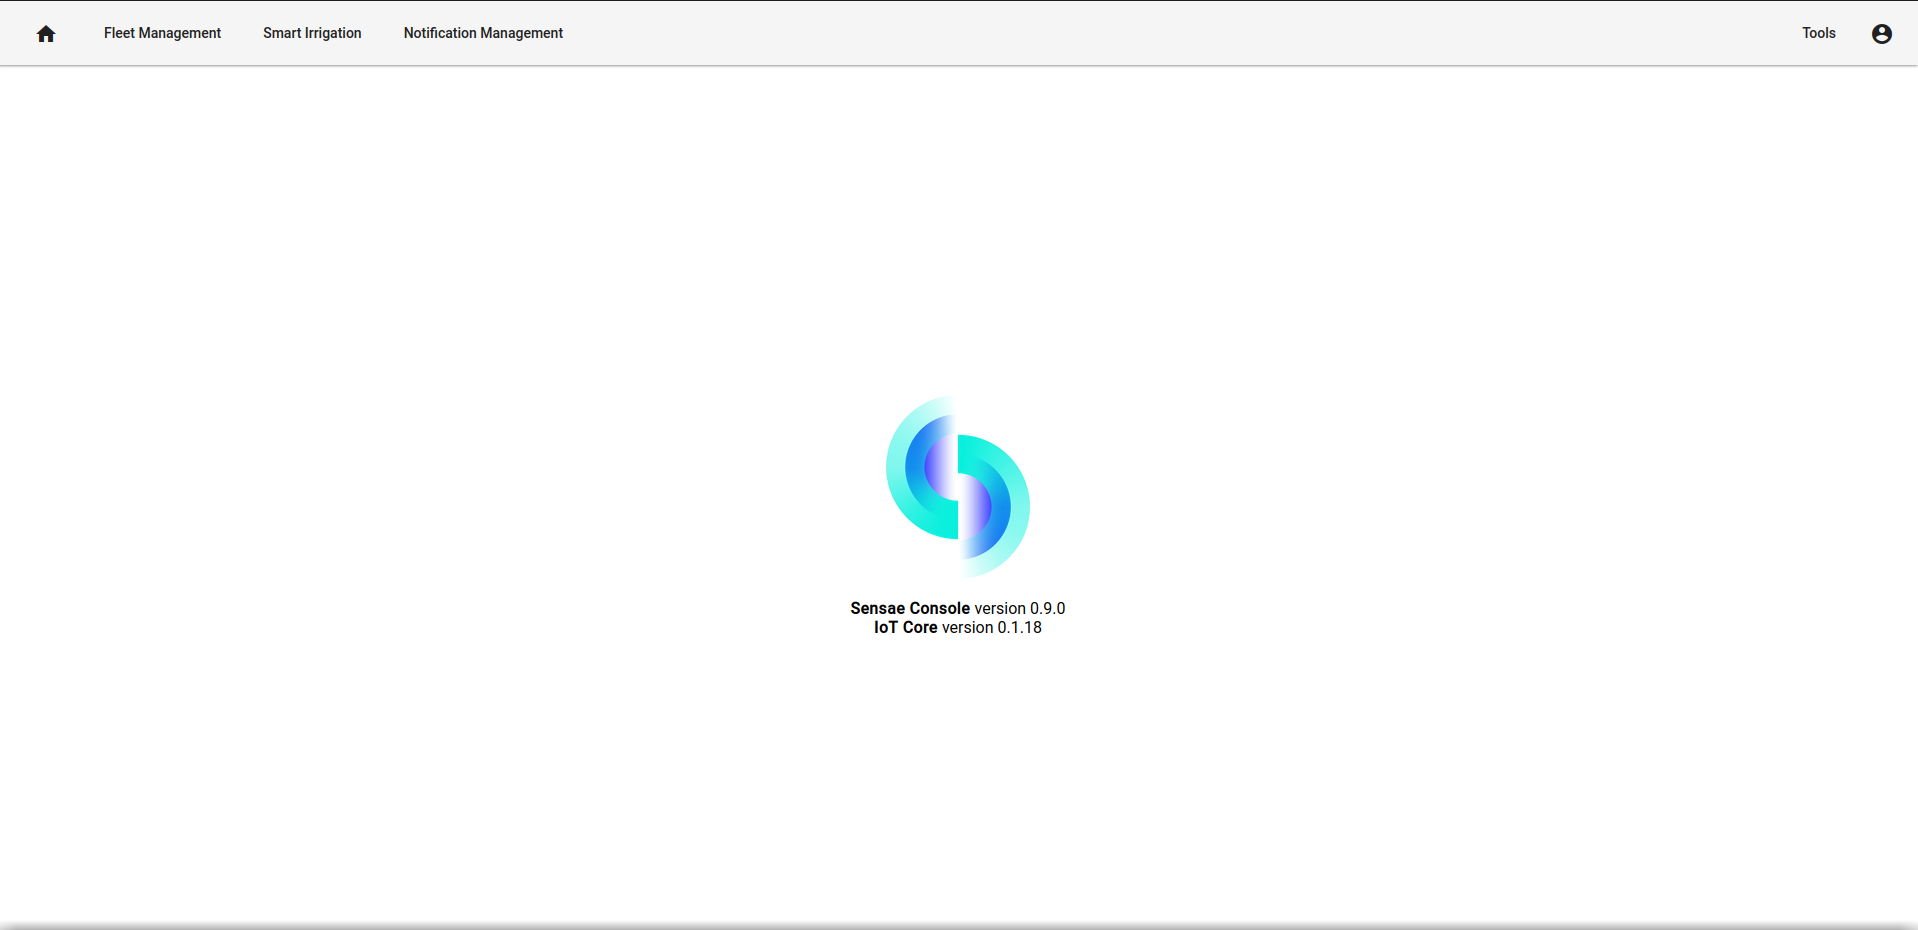
\includegraphics{assets/figures/ui/home.png}
    }
    \caption[Sensae Console Home Page]{Sensae Console Home Page}
    \label{fig:implementation:description:ui:home}
\end{figure}

From this page, if the user has sufficient permissions, he/she can access configuration pages, as an example the \textbf{Device Management Page} is displayed in Figure~\ref{fig:implementation:description:ui:device}.

\begin{figure}[H]
    \centering
    \resizebox{\columnwidth}{!}
    {
       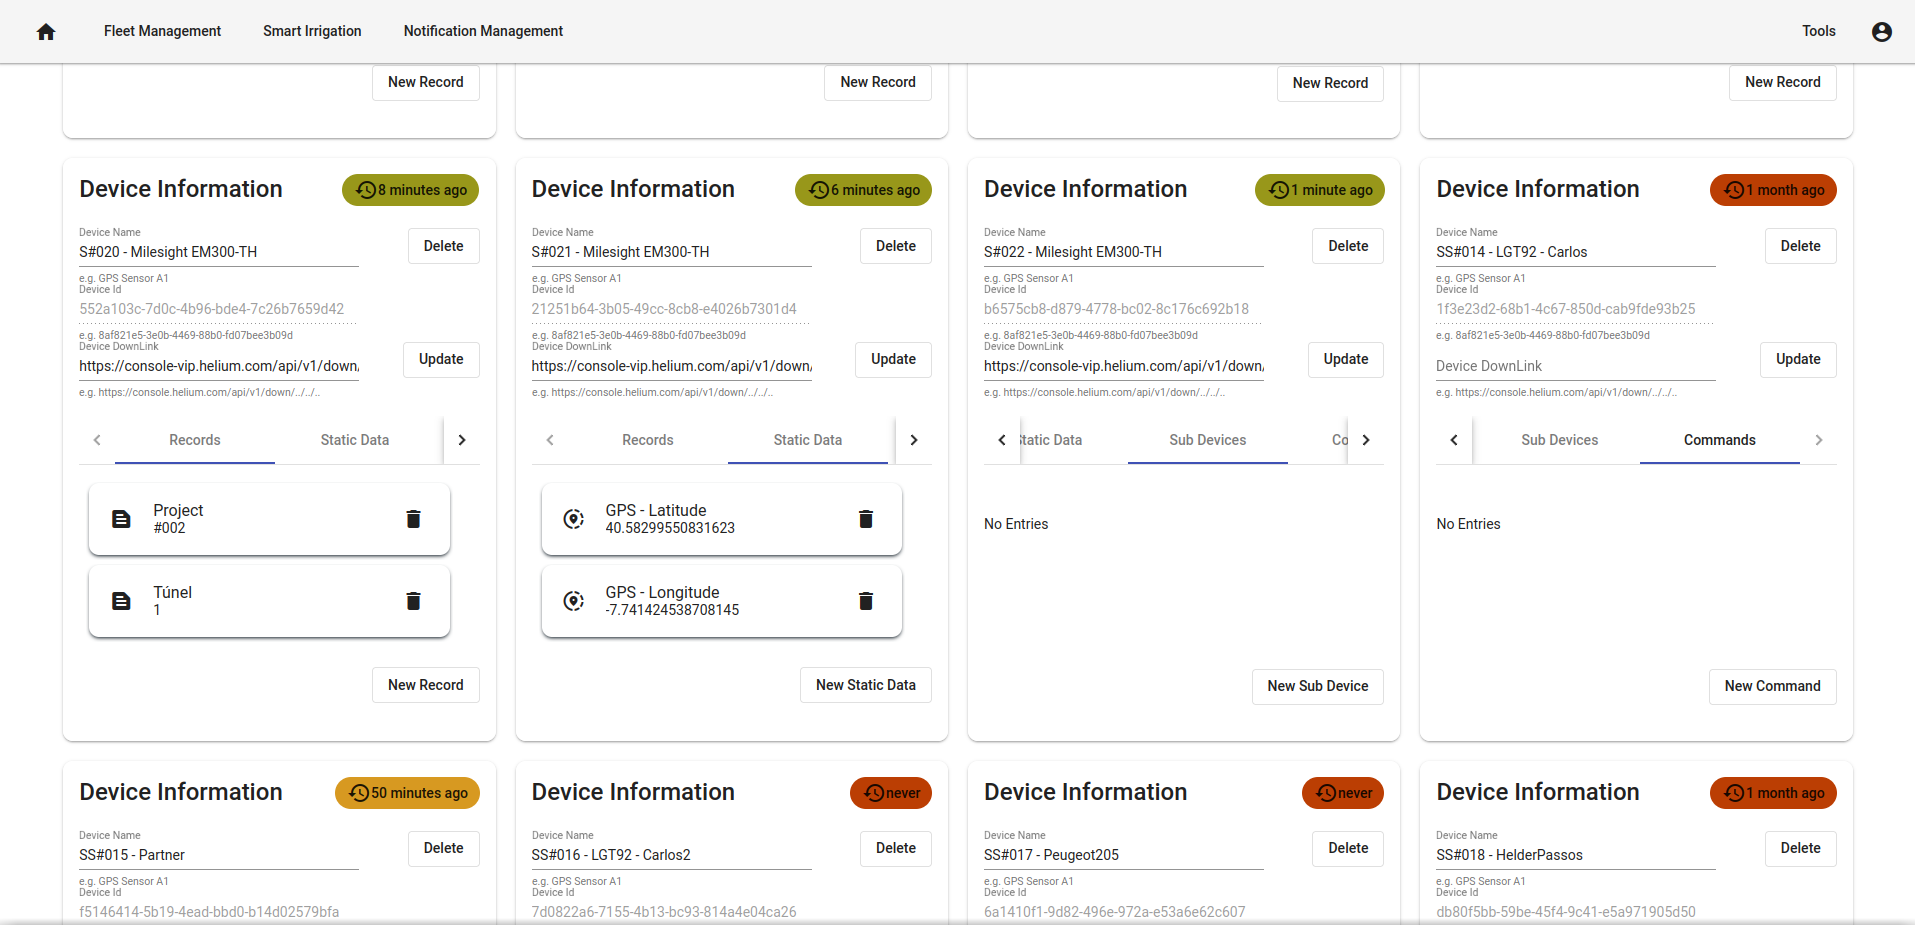
\includegraphics{assets/figures/ui/device-management.png}
    }
    \caption[Sensae Console Device Management Page]{Sensae Console Device Management Page}
    \label{fig:implementation:description:ui:device}
\end{figure}

In this page the user can see when was the last time the device interacted with the platform, create and delete devices and edit the details of each device according to the model presented in Section\nameref{subsubsec:design:domain:bounded_contexts:device} of the \textit{Bounded Contexts}.

From the home page, if the UI Aggregator was configured to fetch external services, one can access those services' pages too, as an example the \textbf{Smart Irrigation Page} is displayed in Figure~\ref{fig:implementation:description:ui:smartirrigation}.
This page presents a map where the user can see, search and create irrigation zones. Device measures are updated in real time via \textit{Websocket}s. The user can also see the irrigation zone details after clicking on it. From there it's possible to open/close valves an see the history of measures of each device.

\begin{figure}[H]
    \centering
    \resizebox{\columnwidth}{!}
    {
       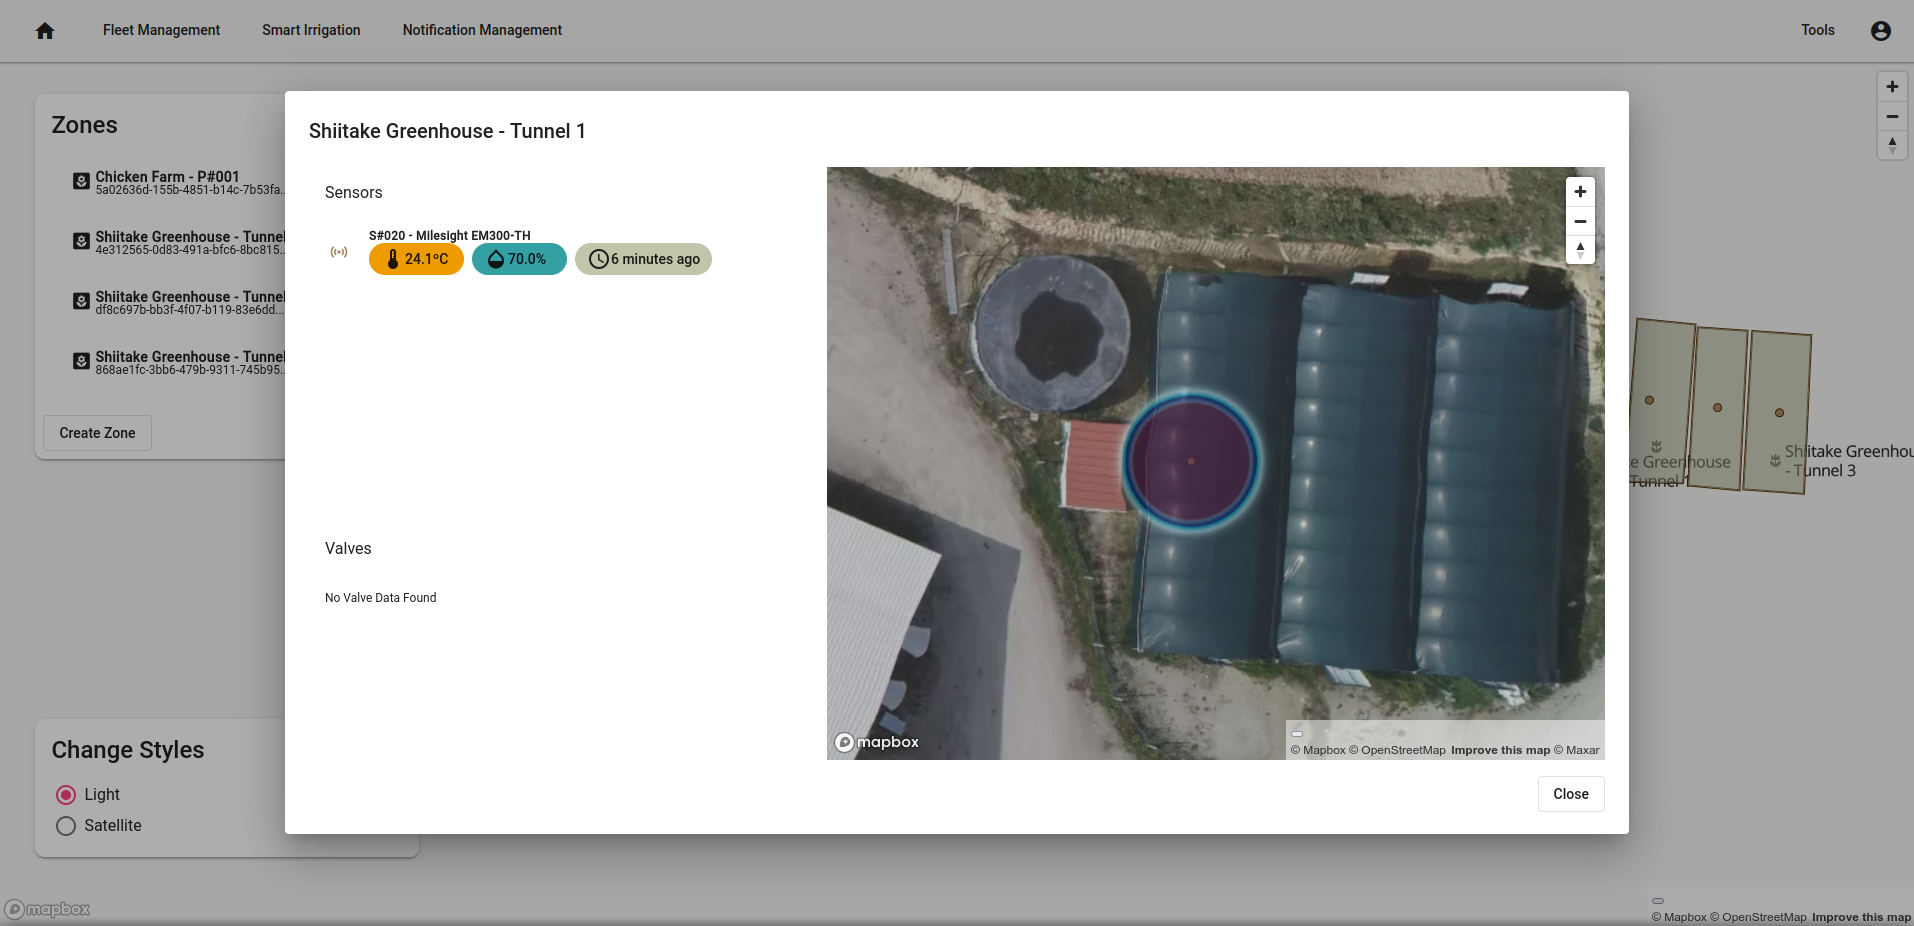
\includegraphics{assets/figures/ui/smart-irrigation.png}
    }
    \caption[Sensae Console Smart Irrigation Page]{Sensae Console Smart Irrigation Page}
    \label{fig:implementation:description:ui:smartirrigation}
\end{figure}

Other relevant pages are presented in the Appendix~\ref{AppendixD}, for Sensae Console, and Appendix~\ref{AppendixD2}, for the Solutions developed.

\subsection{Sensae Console Custom Maps}
\label{subsec:implementation:description:maps}

This section describes how custom maps where built to fit the solution needs. Some costumers facilities were not present in the satellite view of \citetitle{googlemaps} or \citetitle{mapbox}. A custom map, with the missing facilities, was built using satellite images taken with a drone. The images where processed with \citetitle{arcgis} and transformed in \textit{.tiff} files that could be incorporated in the basic satellite layer of \citetitle{mapbox}.

The following image, Figure~\ref{fig:implementation:description:maps:irrig} presents the new map with the costumer facilities in a greener tone than the rest of the map. This map was used to display three greenhouses and a chicken farm that belong to a costumer. This map is currently in use by the Smart Irrigation Service.

\begin{figure}[H]
    \centering
    \resizebox{\columnwidth}{!}
    {
       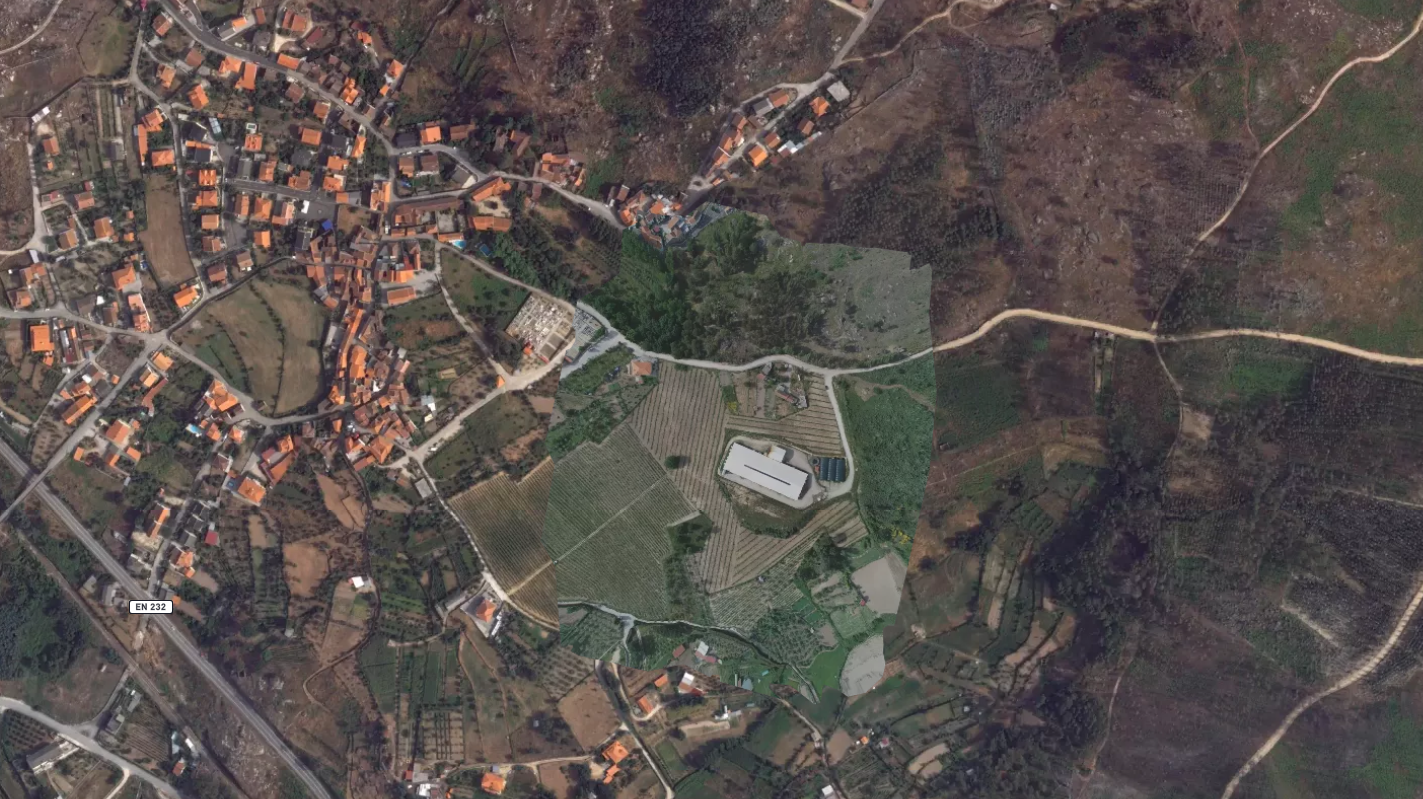
\includegraphics{assets/figures/maps/custom-map.png}
    }
    \caption[Custom Map - Smart Irrigation]{Custom Map - Smart Irrigation}
    \label{fig:implementation:description:maps:irrig}
\end{figure}

The road trajectory mismatch present in the map could be reduced by taking pictures from more angles. \citetitle{arcgis} would create better model with a wider pool of information.

\subsection{Sensae Console Backend API}
\label{subsec:implementation:description:api}

The \textbf{Sensae Console} \gls{API} is served as a \citetitle{graphql} \gls{API}, one for each service/configuration context. This \gls{API} is described with a schema.

As an example the Smart Irrigation API is presented in the Code Sample~\ref{code:implementation:description:api:irrigation}.

\begin{lstlisting}[caption=Smart Irrigation API Schema, label={code:implementation:description:api:irrigation}]
type Subscription {
    data(filters: LiveDataFilter, Authorization: String) : SensorData
}

type Query {
    history(filters: HistoryQueryFilters) : [SensorDataHistory]
    fetchIrrigationZones : [IrrigationZone]
    fetchLatestData(filters: LatestDataQueryFilters): [SensorData]
}

type Mutation {
    createIrrigationZone(instructions: CreateIrrigationZoneCommand) : IrrigationZone
    updateIrrigationZone(instructions: UpdateIrrigationZoneCommand) : IrrigationZone
    deleteIrrigationZone(instructions: DeleteIrrigationZoneCommand) : IrrigationZone
    switchValve(instructions: ValvesToSwitch): Boolean
}
\end{lstlisting}

From the observation of the code sample one can see that:

\begin{itemize}
    \item The \textit{data} function serves new \textit{SensorData} in real-time according to the filters provided in the \textit{filters} parameter;
    \item The textit{data} function uses \textit{Websocket} to operate as a full duplex communication channel. This spec, contrary to the HTTP spec does not account for HTTP Headers, as such the \gls{JWT} that provides the user authentication details has to be sent as a normal parameter and not as an Authorization HTTP Header.
    \item  There are three query type functions. One to fetch the history regarding Irrigation Zones or Devices over a time span. One to fetch the Irrigation Zones. And the last one to fetch the latest data of each device;
    \item There are four mutations, each corresponding to the use cases referenced in Section~\ref{subsubsec:requirements:functional:services:irrigation}.
\end{itemize}

\subsection{Sensae Console Data Ingestion Endpoint}
\label{subsec:implementation:description:ingestion}

The Data Ingestion Endpoint refers to how device data is sent to \textbf{Sensae Console}.

The endpoint corresponds to an HTTP POST verb with the following \gls{URL} schema:

\begin{verbatim}
    https://<ip>:<port>/sensor-data/{channel}/{infoType}/{deviceType}
\end{verbatim}

The endpoint collects the request body and then forwards it with the appropriate routing keys.

The routing keys are created according to the Table~\ref{tab:design:domain:shared_model:routing}. The \textit{infoType} can have two values: ENCODED or DECODED. Depending on this value the message is routed to \textit{Data Decoder Flow} or \textit{Data Processor Flow} as described in Figure~\ref{fig:design:architecture:platform:container:process:diagram:flow}.

The \textit{channel} parameter indicates the final service that it is destine to: \textit{fleet} for Fleet Management Service or \textit{irrigation} for Smart Irrigation Service. If another value is given the message is not routed to any service.

Finally, to ensure that the requests to this endpoint are trustworthy, a secret has to be sent in the Authorization HTTP Header. This secret is defined as a configuration of the \textbf{Sensae Console}, discussed in Section~\ref{subsec:implementation:description:config}.

\subsection{Sensae Console Rule Engine}
\label{subsec:implementation:description:rule}

The rule engine can be access from the \textbf{Rule Management Page} of the UI and, as stated in \nameref{subsubsec:design:domain:bounded_contexts:rule} Bounded Context, it provides a high-level language that can be used to detect anomalies in \textbf{Data Unit}s and turn them into \textbf{Alert}s.

Valid \textbf{Data Unit}s are captured by \textbf{Alert dispatcher Backend} and the inserted in the Rule Engine.

As stated in \nameref{subsec:implementation:decisions:drools}, the rule engine used was \citetitle{drools}. To write rules for \textbf{Sensae Console} one must follow several guidelines.

A \citetitle{drools} rule is composed by conditions, actions and facts.

Facts are inserted in the rule engine. If a fact or group of facts match a condition (\textit{when} section), an action is triggered (\textit{then} section).

The rule engine, is tailored to managers or developers and not for final clients since it can be hard to create meaningfully rules without side effects.

To clarify the guidelines the following Code Samples~\ref{code:implementation:description:rule:sample1}, ~\ref{code:implementation:description:rule:sample2} and \ref{code:implementation:description:rule:sample3} are presented.

The first Code Sample presents the beginning of the rule scenario, where imports and new Facts are created.

\begin{lstlisting}[style=drools, caption=Rule Scenario Example - Part 1, label={code:implementation:description:rule:sample1}]
package rules.project.two;

import pt.sharespot.iot.core.data.model.data.DataUnitReadingsDTO;
import pt.sharespot.iot.core.data.model.DataUnitDTO;
import pt.sharespot.iot.core.data.model.device.records. DeviceRecordEntryDTO;
import pt.sharespot.iot.core.data.model.properties.PropertyName;
import pt.sharespot.iot.core.alert.model.AlertBuilder;
import pt.sharespot.iot.core.alert.model.CorrelationDataBuilder;
import pt.sharespot.iot.core.alert.model.AlertLevel;
import java.util.List;
import java.util.UUID;

global pt.sharespot.iot.core.alert.model.AlertDispatcherService dispatcher;

dialect "mvel"

declare StoveSensor
    @role( event )
    deviceId : UUID
end

declare StoveSensorData
    @role( event )
    deviceId : UUID
    dataId : UUID
    temperature : Float
    humidity : Float
end
\end{lstlisting}

As we can see, from line \textbf{3} to \textbf{9}, classes from \textit{iot-core} are imported into the scenario.
At line \textbf{13} the interface that defines how an alert can be sent is imported for later use.
From line \textbf{17} to \textbf{28} two facts are declared, this can later be used as simple \textit{Java} POJOs. A fact defined with the \textit{event} role means that it occurred at a specific time (upon creation) and can be used for \gls{CEP}.

The following code sample presents a simple rule to store \textit{StoveSensorData} facts in the working memory of \citetitle{drools}.

\begin{lstlisting}[style=drools, caption=Rule Scenario Example - Part 2, label={code:implementation:description:rule:sample2}]
rule "Collect stove sensor data that belongs to Project #002"
    when
        $d : DataUnitDTO(
            getSensorData()
            .hasProperty(PropertyName.AIR_HUMIDITY_RELATIVE_PERCENTAGE),
            getSensorData()
            .hasProperty(PropertyName.TEMPERATURE)
        )
        exists DeviceRecordEntryDTO(
            label == "Project" && content == "#002"
        ) from $d.device.records
        not(StoveSensorData(dataId == $d.dataId))
    then
        StoveSensorData reading = new StoveSensorData();
        reading.setDeviceId($d.device.id);
        reading.setDataId($d.dataId);
        reading.setTemperature($d.getSensorData().temperature.celsius);
        reading.setHumidity($d.getSensorData().airHumidity .relativePercentage);
        insert(reading)
end
\end{lstlisting}

As we can see this rule is composed by two sections, the \textit{when} and \textit{then} sections. In the \textit{when} the following conditions are defined:

\begin{itemize}
    \item The captured DataUnitDTO has AIR HUMIDITY RELATIVE PERCENTAGE and TEMPERATURE measures - lines \textbf{3} to \textbf{8};
    \item The capture DataUnitDTO has a record with a "Project" label and "\#002" content - lines \textbf{9} to \textbf{11};
    \item The DataUnitDTO is not a duplicate fact in the working memory - line \textbf{12}.
\end{itemize}

Once this conditions are meet a \textit{StoveSensorData} is created with all the needed information and then inserted into the working memory - lines \textbf{14} to \textbf{19}.

The following code sample presents a simple rule to dispatch an \textbf{Alert} after some conditions are meet.

\begin{lstlisting}[style=drools, caption=Rule Scenario Example - Part 3, label={code:implementation:description:rule:sample3}]
rule "Dispatch Stove Alarm - Dry Soil Scenario - Project #002"
    when
        $s : StoveSensorData(temperature > 26, humidity < 50)
        not(StoveSensorData(this != $s,
                temperature < 26,
                humidity > 50,
                this after[0s,11m] $s)
        )
    then
        dispatcher.publish(AlertBuilder.create()
                            .setCategory("irrigation")
                            .setSubCategory("drySoilDetected")
                            .setDescription("Project #002 - Device "+ $s.deviceId +" detected low humidity/high temperature")
                            .setLevel(AlertLevel.ADVISORY)
                            .setContext(CorrelationDataBuilder.create()
                                .setDeviceIds($s.deviceId)
                                .setOther("Project #002")
                                .build())
                            .build());
end
\end{lstlisting}

As we can see this rule matches when the same device reports measures of air humidity higher than 50\% and temperature lower then 26 ºC for more than 11 minutes.

Once it matches an Alert is dispatched using the referenced dispatcher in Code Sample~\ref{code:implementation:description:rule:sample1}. The Alert can be created using the builder pattern.

An Alert closely resembles a Notification from the \nameref{subsubsec:design:domain:bounded_contexts:notification} Bounded Context. It also has a category (line \textbf{13}), a sub category (line \textbf{14}), a severity level (line \textbf{16}), a description (line \textbf{15}) and a notification context (lines \textbf{17} to \textbf{20}).

For an \textbf{Alert} to be sent at least the category and sub category parameters have to be set. By default the \textbf{INFORMATION} severity level is used.

In order for services to act upon a received \textbf{Alert}, it has to be associated with a \textit{DeviceId} (this association helps services like \textbf{Smart Irrigation} to know what Valve must be turned on or off), a \textit{DataId} or \textit{Other}.

An \textbf{Alert} is later transformed and store as a Notification, the \textit{DeviceId}s associated to it are used to determine what domains will have access to the Notification. If no \textit{DeviceId}s are associated only the root domain will have access to it.

\subsection{Sensae Console Data Decoders}
\label{subsec:implementation:description:decoder}

As mentioned in the \nameref{subsubsec:design:domain:bounded_contexts:decoder} Bounded Context Section, \textbf{Data decoder}'s purpose is to provide a flexible option to transform inbound data units into something that the system understands.

This happens when a \textbf{Data Unit} has a routing key with the ENCODED info type.

There are certain guidelines to follow in order to create a decoder:

\begin{itemize}
    \item Has to be written in vanilla \textit{javascript};
    \item Has to have an \textit{entry} function with the following signature \textit{function convert(dataUnit)};
    \item Can't import any node function, npm package or reference other scripts.
\end{itemize}

As an example, the Code Sample~\ref{code:implementation:description:decoder:em300th} presents the decoder for the device type EM500-TH\footnote{\href {https://www.milesight-iot.com/lorawan/sensor/em300-th}{Milesight EM300-TH Decoder}}.

\begin{lstlisting}[style=javascript, caption=EM300-TH Data Decoder Example, label={code:implementation:description:decoder:em300th}]
const decodePayload = (payload, port) =>
    ({"0": decoder(base64ToHex(payload), port)});

const base64ToHex = (() => {
    const values = [], output = [];

    return function base64ToHex(txt) {
        if (output.length <= 0) populateLookups();
        const result = [];
        let v1, v2, v3, v4;
        for (let i = 0, len = txt.length; i < len; i += 4) {
            v1 = values[txt.charCodeAt(i)];
            v2 = values[txt.charCodeAt(i + 1)];
            v3 = values[txt.charCodeAt(i + 2)];
            v4 = values[txt.charCodeAt(i + 3)];
            result.push(
                parseInt(output[(v1 << 2) | (v2 >> 4)], 16),
                parseInt(output[((v2 & 15) << 4) | (v3 >> 2)], 16),
                parseInt(output[((v3 & 3) << 6) | v4], 16)
            );
        }
        if (v4 === 64) result.splice(v3 === 64 ? -2 : -1);
        return result;
    };
    function populateLookups() {
        const keys =
            "ABCDEFGHIJKLMNOPQRSTUVWXYZabcdefghijkl mnopqrstuvwxyz0123456789+/=";
        for (let i = 0; i < 256; i++) {
            output.push(("0" + i.toString(16)).slice(-2));
            values.push(0);
        }
        for (let i = 0; i < 65; i++) values[keys.charCodeAt(i)] = i;
    }
})();

function decoder(bytes, port) {
    let decoded = {}, temperature = {}, airHumidity = {}, battery = {};
    for (let i = 0; i < bytes.length;) {
        let channel_id = bytes[i++];
        let channel_type = bytes[i++];
        if (channel_id === 0x01 && channel_type === 0x75) {
            decoded.battery = battery;
            battery.percentage = bytes[i];
            i += 1;
        } else if (channel_id === 0x03 && channel_type === 0x67) {
            decoded.temperature = temperature;
            temperature.celsius = readInt16LE(bytes.slice(i,i+2))/10;
            i += 2;
        } else if (channel_id === 0x04 && channel_type === 0x68) {
            decoded.airHumidity = airHumidity;
            airHumidity.relativePercentage = bytes[i] / 2;
            i += 1;
        } else {
            break;
        }
    }
    return decoded;
}
const readUInt16LE = bytes => (bytes[1] << 8) + bytes[0] & 0xffff;

function readInt16LE(bytes) {
    let ref = readUInt16LE(bytes);
    return ref > 0x7fff ? ref - 0x10000 : ref;
}
const convert = dataUnit => ({
    dataId: dataUnit.uuid,
    reportedAt: dataUnit.reported_at,
    device: {
        id: dataUnit.id,
        name: dataUnit.name,
        downlink: dataUnit.downlink_url,
    },
    measures: decodePayload(dataUnit.payload, dataUnit.port),
});
\end{lstlisting}

As we can see, this code sample decodes an EM300-TH \textbf{Data Unit}. The function \textit{convert} is the one mentioned in the guidelines, it assigns values such as \textit{id}, \textit{name}, \textit{reported\_at}, \textit{downlink\_url}, \textit{uuid} to its correct place and calls the function \textit{decodePayload} to gather the device measures. The \textit{decodePayload} stores every measure in the \textit{controller} key - value \textit{0}. The function \textit{base64ToHex} is the function that reads a Base 64 string and transforms it into a Hex Array - to reduce bandwidth the device normally encodes and sends data as a base 64 string. The function \textit{decoder}, \textit{readInt16LE} and \textit{readUInt16LE} were adapted from the TTN decoder\footnote{\href {https://www.milesight-iot.com/lorawan/sensor/em300-th}{Milesight EM300-TH Decoder}} of this device.

\subsection{Sensae Console Database Configuration}
\label{subsec:implementation:description:database}

The solution designed relies on various databases, and as discussed in Section~\ref{subsubsec:implementation:decisions:database:relational} some are relational databases. \citetitle{postgressql} and most databases of this data-model type require a database schema. For this solution the schema of each database is defined in a \textit{sql} file that is executed at the start of the database, only if no data is found.

Further database schema migrations are preformed using custom \gls{SQL} scripts when needed. In the future, once more instance of \textbf{Sensae Console} are deployed, the use of liquidbase or flyway is preferred.

The following Code Sample~\ref{code:implementation:description:database:file} exemplifies the content of this scripts.

\begin{lstlisting}[language=SQL, caption=Initialization Script Segment for Data Processor Database, label={code:implementation:description:database:file}]
create table if not exists public.transformation
(
    persistence_id bigint generated by default as identity
        primary key,
    device_type    varchar(255)
        constraint unique_type_constrain
            unique
);

create table if not exists public.property_transformation
(
    persistence_id                bigint generated by default as identity (maxvalue 2147483647)
        primary key,
    value                         integer           not null,
    old_path                      varchar(255),
    transformation_persistence_id bigint
        constraint ref_transformation_constrain
            references public.transformation,
    sub_sensor_id                 integer default 0 not null
);
\end{lstlisting}

This script defines two simple tables, \textit{transformation} and \textit{property\_transformation}, following the concepts defined in Section~\ref{subsubsec:design:domain:bounded_contexts:processor}.

Apart from the schema, the \textbf{Identity Management Database} also requires the following bootstrap data, as implied in \nameref{subsubsec:design:domain:bounded_contexts:identity} Bounded Context Section:

\begin{itemize}
    \item Root domain;
    \item Public domain;
    \item Unallocated Root domain;
    \item Anonymous Tenant account;
    \item Admin Tenant account;
\end{itemize}

This data is inserted using the following function, Code Sample~\ref{code:implementation:description:database:function}:

\begin{lstlisting}[language=SQL, caption=Bootstrap function for Identity Management Database, label={code:implementation:description:database:function}]
CREATE FUNCTION public.init_domains ()
RETURNS varchar(255) AS $root_oid$
    DECLARE
        root_oid varchar(255) := gen_random_uuid();
        public_oid varchar(255) := gen_random_uuid();
        unallocated_oid varchar(255) := gen_random_uuid();
    BEGIN
        INSERT INTO public.domain (name, oid, path)
        VALUES ('root', root_oid, ARRAY[root_oid]);
        INSERT INTO public.domain (name, oid, path)
        VALUES ('public', public_oid, ARRAY[root_oid, public_oid]);
        INSERT INTO public.domain (name, oid, path)
        VALUES ('unallocated', unallocated_oid, ARRAY[root_oid, unallocated_oid]);
        INSERT INTO public.tenant (name, oid, phone_number, email, domains)
        VALUES ('Anonymous', gen_random_uuid(), '', '', ARRAY[public_oid]);
        INSERT INTO public.tenant (name, oid, phone_number, email, domains)
        VALUES ('Admin', gen_random_uuid(), '', '$SENSAE_ADMIN_EMAIL', ARRAY[root_oid]);
        RETURN root_oid;
    END;
$root_oid$ LANGUAGE plpgsql;

select public.init_domains();

DROP FUNCTION public.init_domains;
\end{lstlisting}

This function starts by declaring three \gls{UUID} - lines \textbf{4} to \textbf{6} - that will later be used to populate the domain's \textit{path} and the tenant's \textit{domains} - lines \textbf{7} to \textbf{17}. In the end the function is executed and then removed to ensure that it isn't executed again.

In line \textbf{17}, the variable \textbf{\$SENSAE\_ADMIN\_EMAIL} is replace by a valid email before building the database container with the full script. This variable configuration is discussed in the Section~\ref{subsec:implementation:description:config}.

\subsection{Sensae Console Containerization}
\label{subsec:implementation:description:docker}

The section describes how \textbf{Sensae Console} is containerized with docker.
As explained in Section~\ref{subsec:implementation:decisions:docker}, the author choose to containerize the solution.

The following Code Samples describe how each container mentioned during the Design Chapter are packaged. To simplify, only three distinct samples will be presented.

The first sample, Listing~\ref{code:implementation:description:docker:frontend}, refers to UI Aggregator and is similar to all other frontend containers.

\begin{lstlisting}[caption=Dockerfile for UI Aggregator Frontend, label={code:implementation:description:docker:frontend}]
FROM node:18-alpine AS build
WORKDIR /workspace
COPY package.json ./
COPY . .
RUN npm install
RUN npm run nx build ui-aggregator --omit=dev

FROM nginx:1.23.1
COPY apps/ui-aggregator/nginx/nginx.conf /etc/nginx/conf.d/default.conf
COPY --from=build /workspace/dist/apps/ui-aggregator /usr/share/nginx/html
\end{lstlisting}

This Dockerfile contains two stages to reduce the size of the final image. The first stage, lines \textbf{1} to \textbf{6}, builds the project. The second one, containing only \citetitle{nginx} and the code that was previously built, is used to serve the UI Aggregator Frontend and route requests. The \citetitle{nginx} configuration file at line \textbf{9} is discussed in the \ref{subsec:implementation:description:nginx} Section.

The second sample, Listing~\ref{code:implementation:description:docker:spring}, refers to \textbf{Fleet Management Backend} and is similar to all backend containers in the Configuration Scope or External Services.

\begin{lstlisting}[caption=Dockerfile for Fleet Management Backend, label={code:implementation:description:docker:spring}]
FROM maven:3.8.5-openjdk-18 AS build
WORKDIR /app
# copy all pom.xml to pull only external dependencies
COPY application/pom.xml application/pom.xml
COPY domain/pom.xml domain/pom.xml
COPY infrastructure/boot/pom.xml infrastructure/boot/pom.xml
COPY infrastructure/endpoint/pom.xml infrastructure/endpoint/pom.xml
COPY infrastructure/persistence/pom.xml infrastructure/persistence/pom.xml
COPY infrastructure/persistence/questdb/pom.xml infrastructure/persistence/questdb/pom.xml
COPY infrastructure/endpoint/graphql/pom.xml infrastructure/endpoint/graphql/pom.xml
COPY infrastructure/endpoint/amqp/pom.xml infrastructure/endpoint/amqp/pom.xml
COPY infrastructure/pom.xml infrastructure/pom.xml
COPY pom.xml pom.xml
# build all external dependencies
RUN mvn -B -e -C org.apache.maven.plugins:maven-dependency-plugin:3.1.2:go-offline -DexcludeArtifactIds=fleet-management-backend,application,domain,infrastructure,endpoint,graphql,boot,amqp,questdb

COPY . .
RUN mvn clean package

FROM openjdk:17
WORKDIR /app
COPY --from=build /app/infrastructure/boot/target/fleet-management-backend.war /app
CMD ["java", "-jar", "fleet-management-backend.war"]
\end{lstlisting}

This sample also presents a multi-stage Dockerfile. The first stage, line \textbf{1} to \textbf{18} builds the project with Maven. All \textit{pom.xml} files and dependencies are added first to reduce build time during development, since these change less that the code written. The second stage is the one that runs the  service. It only contains the \gls{JDK} and the compiled application.

The third sample, Listing~\ref{code:implementation:description:docker:quarkus}, refers to \textbf{Device Commander} and is similar to all backend containers in the Data Flow Scope.

\begin{lstlisting}[caption=Dockerfile for Device Commander, label={code:implementation:description:docker:quarkus}]
FROM quay.io/quarkus/ubi-quarkus-native-image:22.1-java17 AS build
COPY --chown=quarkus:quarkus mvnw /code/mvnw
COPY --chown=quarkus:quarkus .mvn /code/.mvn
COPY --chown=quarkus:quarkus pom.xml /code/
USER quarkus
WORKDIR /code
RUN ./mvnw -B org.apache.maven.plugins:maven-dependency-plugin:3.1.2:go-offline
COPY src /code/src
RUN ./mvnw package -Pnative

FROM quay.io/quarkus/quarkus-micro-image:1.0
WORKDIR /work/
COPY --from=build /code/target/runner /work/application

# set up permissions for user `1001`
RUN chmod 775 /work /work/application \
    && chown -R 1001 /work \
    && chmod -R "g+rwX" /work \
    && chown -R 1001:root /work

EXPOSE 8080
USER 1001

CMD ["./application", "-Dquarkus.http.host=0.0.0.0"]
\end{lstlisting}

This sample, once again, is also a multi-stage Dockerfile. It was adapted from the one generated by \citetitle{quarkus} when setting up the application. In the first stage the application is built with a \citetitle{graalvm} native-image - lines \textbf{1} to \textbf{9}. This allows the image to run without \gls{JVM}. The second stage runs the service after setting user permissions, so that the process doesn't run as root, at lines \textbf{17} to \textbf{20}.

\subsection{Sensae Console Orchestration}
\label{subsec:implementation:description:compose}

As described in Section~\ref{par:design:architecture:platform:container:physical}, \citetitle{dockercompose} was the tool used to orchestrate the whole solution, the \textbf{Sensae Console} and External Services. This tool consumes a configuration file to know what containers, and their configurations, are needed. The complete configuration file for production is vast, a summarized version will be presented containing only the \textbf{Data Processor} Context' related containers.

\begin{lstlisting}[style=yaml, caption=Docker Compose Configuration File for Production, label={code:implementation:description:compose:file}]
services:
  data-processor-frontend:
    build:
      dockerfile: docker/data-processor-frontend/Dockerfile
      context: frontend-services
    image: data-processor-frontend
    volumes:
      - /etc/letsencrypt:/etc/letsencrypt/
      - /etc/nginx/ssl:/etc/nginx/ssl/
    networks:
      - sensae-network
    ports:
      - 443
    depends_on:
      - data-processor-master-backend
  data-processor-master-backend:
    build: backend-services/data-processor-master-backend
    image: data-processor-master-backend
    volumes:
      - ./secrets/keys:/etc/ssh/app
    environment:
      spring_profiles_active: prod
    env_file:
      - ./secrets/prod/data-processor-master-backend.env
    networks:
      - sensae-network
    ports:
      - 8080
  data-processor-database:
    build: databases/data-processor-database
    container_name: data-processor-database
    env_file:
      - ./secrets/prod/data-processor-database.env
    networks:
      - sensae-network
    ports:
      - 5482:5432
    volumes:
      - ./databases-data/prod/data-processor-database:/var/lib/postgresql/data/
  data-processor-flow:
    build: backend-services/data-processor-flow
    image: sensae/data-processor-flow
    env_file:
        - ./secrets/prod/data-processor-flow.env
    networks:
        - sensae-network
networks:
  sensae-network:
\end{lstlisting}

The following conclusions can be observed:

\begin{itemize}
    \item This context, similar to other contexts, is composed by four containers, a Frontend - \textit{data-processor-frontend}, a Configuration Backend - \textit{data-processor-master-backend}, a Database - \textit{data-processor-database}, and a Data Flow Backend - \textit{data-processor-flow};
    \item All services communicate in the same network - \textit{sensae-network};
    \item All services have instructions on how to build them;
    \item Various configuration files are loaded, e.g. in lines \textbf{19} to \textbf{20} and \textbf{28} to \textbf{31}, this files content will be discussed in the \nameref{subsec:implementation:description:config} Section;
    \item The Frontend has two volumes mapped, one loads the \textit{letsencrypt} configuration file for \citetitle{nginx} and the other loads the SSL certificate - lines \textbf{7} to \textbf{9}.
    \item The Configuration Backend needs to validate the authentication tokens received, for that, it has access to the public key that pairs the private key used to created then in \textbf{Identity Management Backend} - line \textbf{19} - \textbf{20};
    \item The database exposes a port to the host so that it can be managed remotely - lines \textbf{36} to \textbf{37};
    \item The database maps its data to a directory in the host, so that data is persisted between server restarts - lines \textbf{38} to \textbf{39};
    \item The Data Flow container doesn't need to expose any port since it only exchanges information with the message broker;
\end{itemize}

\subsection{Sensae Console Reverse Proxy Configuration}
\label{subsec:implementation:description:nginx}

This section reveals how \citetitle{nginx} is configured for all frontend containers in the solution. As an example, the Listing~\ref{code:implementation:description:nginx:irrig}, describes the \textbf{Smart Irrigation Frontend}.

\begin{lstlisting}[caption=Configuration File for Production Environment, label={code:implementation:description:nginx:irrig}]
server {

    server_name localhost;

    listen 443 ssl;

    ssl_certificate /etc/nginx/ssl/nginx.crt;
    ssl_certificate_key /etc/nginx/ssl/nginx.key;

    root        /usr/share/nginx/html;

    index       index.html index.htm;

    include /etc/letsencrypt/options-ssl-nginx.conf;

    location ~ .*remoteEntry.js$ {
        expires -1;
        add_header 'Cache-Control' 'no-store, no-cache, must-revalidate, proxy-revalidate, max-age=0';
    }

    location /smart-irrigation/graphql {
        proxy_pass http://smart-irrigation-backend:8080/graphql;
        proxy_set_header x-forwarded-prefix /smart-irrigation/graphql;
        proxy_set_header Host $host;
        proxy_set_header x-forwarded-host $host;
        proxy_redirect off;
        proxy_set_header x-forwarded-port 443;
        proxy_set_header x-forwarded-proto https;
    }

    location /smart-irrigation/subscriptions {
        proxy_pass http://smart-irrigation-backend:8080/subscriptions;
        proxy_set_header x-forwarded-prefix /smart-irrigation/subscriptions;
        proxy_http_version 1.1;
        proxy_set_header Upgrade $http_upgrade;
        proxy_set_header Connection "Upgrade";
        proxy_set_header Host $host;
        proxy_read_timeout 6000;
        proxy_send_timeout 6000;
        proxy_redirect off;
        proxy_set_header x-forwarded-port 443;
        proxy_set_header x-forwarded-proto https;
    }

    location / {
        try_files $uri $uri/ /index.html;
    }

    if ($scheme != "https") {
        return 301 https://$host$request_uri;
    } # managed by Certbot
}
\end{lstlisting}

The following conclusions can be inferred:

\begin{itemize}
    \item It only exposes the HTTPS port - line \textbf{4} and lines \textbf{49} to \textbf{51};
    \item It loads the SSL certificates mapped in the \citetitle{dockercompose} file - lines \textbf{7} and \textbf{8};
    \item It uses the \textit{letsencrypt} configuration - line \textbf{14};
    \item The \textit{remoteEntry} file, responsible for providing the entry point to the service in a Micro Frontend environment, is never cached in the client browser since it points to the current compiled version of the service. If this file is cached, the updated version of a micro frontend, can only be accessed by the client browser once the local cache is cleaned up - lines \textbf{16} to \textbf{19};
    \item The \citetitle{graphql} endpoint is defined as a reverse proxy endpoint. Requests made to \textit{/smart-irrigation/graphql} are routed to \textit{http://smart-irrigation-backend:8080/graphql}. It doesn't use a secure connection, HTTPS, since this communication already happens inside the docker network where man in the middle attacks are disregarded - lines \textbf{21} to \textbf{29};
    \item The \citetitle{graphql} subscription endpoint is also defined, this type of connection, \textit{Websocket}, requires the use of HTTP version 1.1 and the two Headers presented at lines \textbf{34} to \textbf{36};
    \item All other requests are handled in lines \textbf{45} to \textbf{47}.
\end{itemize}

\subsection{Sensae Console Configuration Files}
\label{subsec:implementation:description:config}

This section describes how a \textbf{Sensae Console} and External Services are configured. One of the problems that arise from a microservice architecture is how to maintain all configurations for each container developed and configured. Following the \citetitle{confcentral}, all configurations are defined via configuration files that support three environments: \textit{dev}, \textit{test} and \textit{prod}.

This configurations are defined, for each environment, in a single file. This file, Listing~\ref{code:implementation:description:config:file}, has the following structure:

\begin{lstlisting}[language=bash, style=bash, caption=Configuration File for Production Environment, label={code:implementation:description:config:file}]
export SENSAE_MAPBOX_ACCESS_TOKEN=
export SENSAE_MAPBOX_SIMPLE_STYLE=
export SENSAE_MAPBOX_SATELLITE_STYLE=
export SENSAE_BROKER_USERNAME=
export SENSAE_BROKER_PASSWORD=
export SENSAE_COMMON_DATABASE_PASSWORD=
export SENSAE_DATA_STORE_USER_PASSWORD=
export SENSAE_DATA_STORE_ROOT_PASSWORD=
export SENSAE_AUTH_PATH_PUB_KEY=
export SENSAE_AUTH_PATH_PRIV_KEY=
export SENSAE_AUTH_ISSUER=
export SENSAE_AUTH_AUDIENCE=
export SENSAE_DATA_AUTH_KEY=
export SENSAE_AUTH_EXTERNAL_MICROSOFT_AUDIENCE=
export SENSAE_AUTH_EXTERNAL_GOOGLE_AUDIENCE=
export SENSAE_SMS_TWILIO_ACCOUNT_SID=
export SENSAE_SMS_TWILIO_AUTH_TOKEN=
export SENSAE_SMS_SENDER_NUMBER=
export SENSAE_SMS_ACTIVATE=
export SENSAE_EMAIL_SENDER_ACCOUNT=
export SENSAE_EMAIL_SUBJECT=
export SENSAE_EMAIL_SENDER_PASSWORD=
export SENSAE_EMAIL_SMTP_HOST=
export SENSAE_EMAIL_SMTP_PORT=
export SENSAE_EMAIL_ACTIVATE=
export SENSAE_PROD_PUBLIC_DOMAIN=
export SENSAE_ADMIN_EMAIL=
\end{lstlisting}

This file variables are then passed on to each container's environment configuration file with the help of a script. The Code Sample~\ref{code:implementation:description:config:script} sheds a light on how the script propagates the configurations.

\begin{lstlisting}[language=bash, style=bash, caption=Configuration Propagation Script, label={code:implementation:description:config:script}]
#!/usr/bin/sh

ROOT_DIR=$(git rev-parse --show-toplevel)

cd "$ROOT_DIR"/project || exit

. ./secrets/prod.conf

SECRET_BACK=secrets/templates/prod/backend-services
SECRET_FRONT=secrets/templates/prod/frontend-services
SECRET_DB=secrets/templates/prod/databases

BACK_PREFIX=secrets/prod
FRONT_PREFIX=frontend-services/apps
FRONT_SUFFIX=src/environments/environment.prod.ts

envsubst < $SECRET_BACK/alert-dispatcher-backend.env > \
     $BACK_PREFIX/alert-dispatcher-backend.env
# and all other backend services
envsubst < $SECRET_BACK/data-validator.env >
     $BACK_PREFIX/data-validator.env

envsubst < $SECRET_FRONT/device-management-frontend.ts > \
 $FRONT_PREFIX/device-management-frontend/$FRONT_SUFFIX
# and all other frontend services
envsubst < $SECRET_FRONT/ui-aggregator.ts > \
 $FRONT_PREFIX/ui-aggregator/$FRONT_SUFFIX

envsubst < secrets/templates/prod/message-broker/message-broker.env > \
 $BACK_PREFIX/message-broker.env

envsubst < $SECRET_DB/data-decoder-database.env > \
 $BACK_PREFIX/data-decoder-database.env
# and all other databases
envsubst < $SECRET_DB/rule-management-database.env > \
 $BACK_PREFIX/rule-management-database.env
\end{lstlisting}

In the future, as more isolated deployments are made, a tool such as \citetitle{vault} should be integrated in the solution.

\subsection{Solutions - External Services}
\label{subsec:implementation:description:services}

This section discusses how external services interact with the Sensae \gls{API}, this was briefly mentioned in Section~\ref{subsubsec:design:domain:shared_model:routing}.

In order to provide an easy to understand integration with the platform, the routing keys concept was introduced. The idea, from the point of view of someone developing a service, is to start by defining what type of information that service should capture.

The two types of information a service usually needs are: (i) \textbf{Data Unit}s and (ii) \textbf{Alert}s. Each of this information are defined by their routing keys as described in Table~\ref{tab:design:domain:shared_model:routing}.

A service can also publish \textbf{Command}s.

The following sub sections will detail each service information needs.

\subsubsection{Fleet Management Service}
\label{subsubsec:implementation:description:services:fleet}

The focus of this service was to simply collect the location of the costumers' fleet since the company was given no permission to access the vehicles' \gls{OBD} System. Access to the \gls{OBD} System would provide a deeper knowledge regarding the vehicles' conditions.

Therefore, this service captures information of a single type (and doesn't publish any Command):

\textbf{Data Topic}: \textit{'processed'}, \textit{'correct'}, with \textit{'defined ownership'} and \textit{'device information'} data unit with \textit{'gps'} readings in the channel \textit{'fleet'}.

At a high-level view, this service only requires \gls{GPS} data sent to the \textit{'fleet'} channel.

\subsubsection{Notification Management Service}
\label{subsubsec:implementation:description:services:notification}

The focus of this service was to simply showcase and dispatch the alerts sent by \textbf{Sensae Console}. A simple rule scenario for Indoor Fire Detention was then created based on tests performed on a costumer's facilities (Appendix \ref{AppendixH}). The rule scenario was based on the following metrics: CO2 \gls{PPM}, Air humidity and Air Temperature.

This service captures information of a single type (and doesn't publish any Command):

\textbf{Alert Topic}: alerts with \textit{'defined ownership'}.

At a high-level view, this service requires all alerts that already have a \textit{'defined ownership'}.

It is divided in two backend containers (as described in Figure~\ref{fig:design:architecture:solutions:containers:logical:noti}) that subscribe to the same information but handle it differently.

\subsubsection{Smart Irrigation Service}
\label{subsubsec:implementation:description:services:irrigation}

The focus of this service was on the two most common types of agriculture mentioned in literature, outdoor and greenhouse, according to \cite{garcia2020iot}.

The Greenhouse agriculture type collects two measures: (i) Air Temperature and (ii) Air Humidity, the Outdoor agriculture also collects two measures: (i) Luminosity and (ii) Soil Moisture. Both rely on a irrigation system that can be activated and deactivated remotely, like a simple switch, to regulate the monitured environment.

The measures to capture were chosen according to costumers' sugestions and \cite{garcia2020iot} that states that the Soil moisture, Air Temperature, Air Humidity and Luminosity parameters are the most common monitured parameters in papers that propose an irrigaiton system. 

This service captures information of the given types:

\begin{itemize}
    \item \textbf{Data Topic}: \textit{'processed'}, \textit{'correct'}, with \textit{'defined ownership'} and \textit{'device information'} data unit with \textit{'gps'} and \textit{'trigger'} readings in the channel \textit{'irrigation'} (for valves);
    \item \textbf{Data Topic}: \textit{'processed'}, \textit{'correct'}, with \textit{'defined ownership'} and \textit{'device information'} data unit with \textit{'gps'}, \textit{'temperature'} and \textit{'air humidity'} readings in the channel \textit{'irrigation'} (for green house sensors);
    \item \textbf{Data Topic}: \textit{'processed'}, \textit{'correct'}, with \textit{'defined ownership'} and \textit{'device information'} data unit with \textit{'gps'}, \textit{'illuminance'} and \textit{'soil moisture'} readings in the channel \textit{'irrigation'} (for park sensors);
    \item \textbf{Alert Topic}: alerts with the category \textit{'smartIrrigation'} and sub category \textit{'drySoil'} (to open all valves in a garden);
    \item \textbf{Alert Topic}: alerts with \textit{'defined ownership'}, the category \textit{'smartIrrigation'} and sub category \textit{'moistSoil'} (to close all valves in a garden);
    \item \textbf{Alert Topic}: alerts with \textit{'defined ownership'}, the category \textit{'smartIrrigation'} and sub category \textit{'valveOpenForLengthyPeriod'} (to close that specific valve).
\end{itemize}

It then publishes Commands to close or open valves. The service can only issue a command if the Data Unit sent by the valve refers two commands, one to open and another to close the valve. This commands, usually defined in the \textbf{Device Management Page}, and mentioned in the \nameref{subsubsec:design:domain:bounded_contexts:device} Bounded Context, need to have the \textit{CommandId} value as \textit{'openValve'} or \textit{'closeValve'}.

At a high-level view, this service requires data from \textit{Park} sensors, \textit{Green Houses} and \textit{Valves} that flow in the \textit{'irrigation'} channel. It captures Alerts to decide when to open or close Valves by sending specific Commands.

\subsection{Sensae Console Device Integration}
\label{subsec:implementation:description:sensor}

This section describes how devices can be connected to \textbf{Sensae Console}. As stated in Section~\ref{sec:requirements:non_functional}, the service that must be used to communicate with devices is \citetitle{helium}. This solution works with other platforms, such as Azure IoT Hub, since it provides an agnostic data ingestion endpoint as stated in Section~\ref{subsec:implementation:description:ingestion}.

Virtually any device can be integrated, via \citetitle{helium}, with \textbf{Sensae Console}. To do so, one needs to register new devices in \citetitle{helium}, for example via \gls{OTAA}. Then create a Custom HTTP Integration, following the Section~\ref{subsec:implementation:description:ingestion} instructions.

The Figure~\ref{fig:implementation:description:sensor:integration} presents an example of the custom integration for the EM300-TH Device.

\begin{figure}[H]
    \centering
    \resizebox{\columnwidth}{!}
    {
       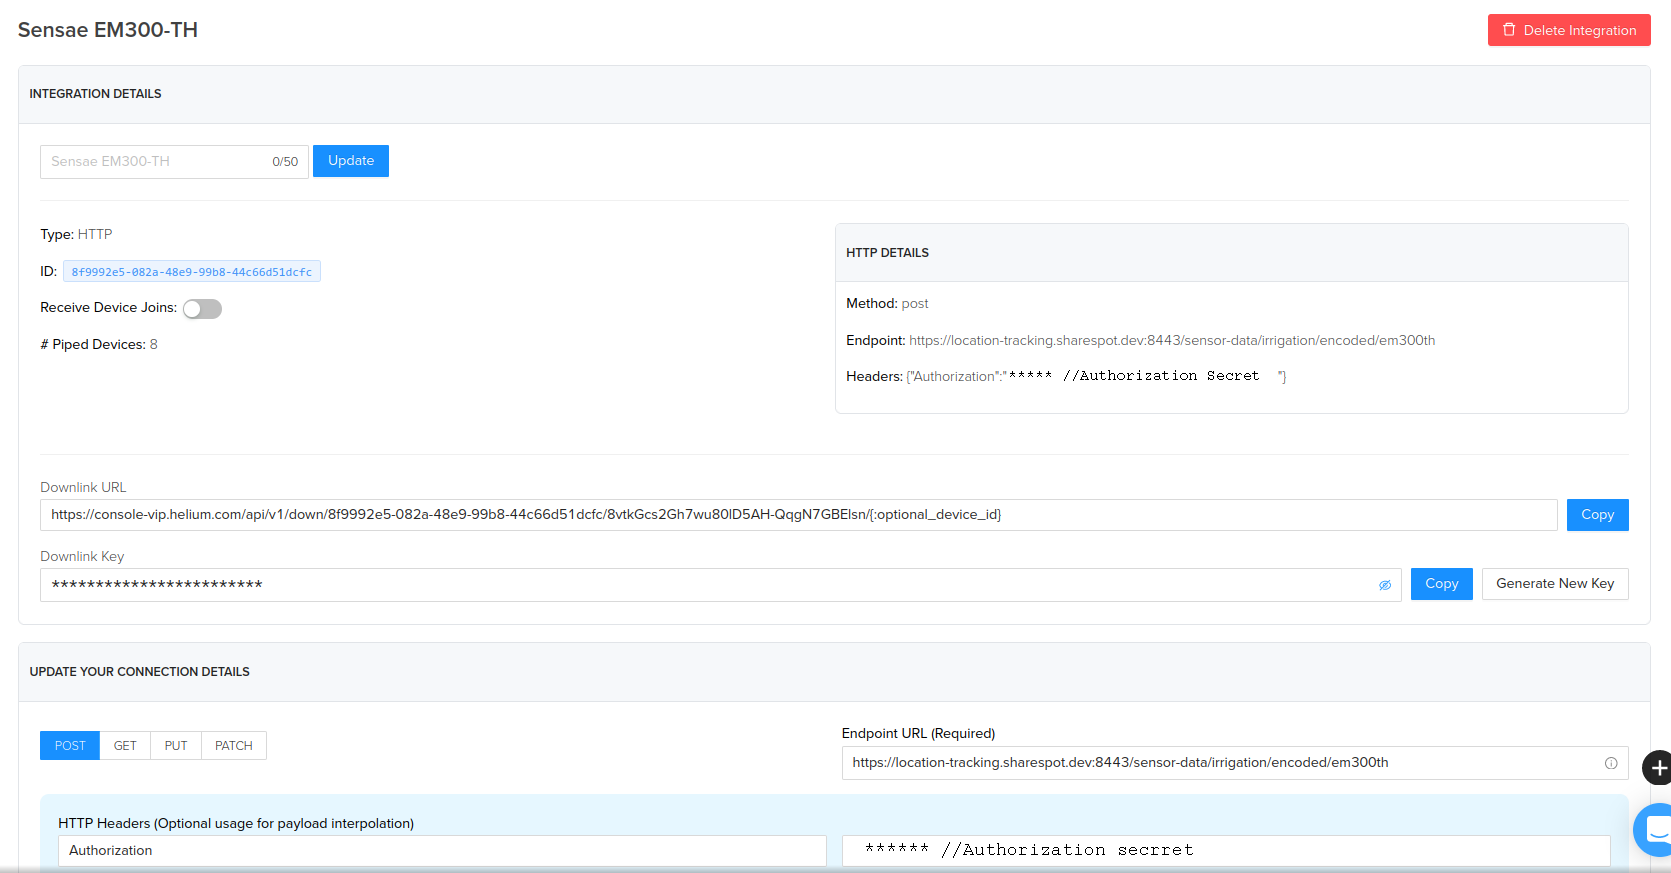
\includegraphics{assets/figures/sensor/integration.png}
    }
    \caption[Helium Custom Integration Page]{Helium Custom Integration Page}
    \label{fig:implementation:description:sensor:integration}
\end{figure}

Finally, in the \citetitle{helium} flows page, connect the registered device to the custom integration.

This method will require the user to register the endpoint with the \textit{encoded} type and write a \textbf{Data Decoder} in \textbf{Sensae Console} to translate the payload sent by the device though \citetitle{helium}.

If the user intends to use the \textbf{Data Processor}, he/she needs to:

\begin{itemize}
    \item Register the endpoint with the \textit{decoded} type;
    \item Define a \textbf{Data Processor} in \textbf{Sensae Console} to map the payload sent by \citetitle{helium};
    \item Write the decoder in \citetitle{helium} - in the \textit{Function} page;
    \item Link the device to the \textit{Function} in \citetitle{helium};
    \item Link the \textit{Function} to the custom integration;
\end{itemize}

\section{Testing}
\label{sec:implementation:testing}

According to \cite{booktest}: ``Software testing is the activity of running a series of dynamic executions of software programs after the software source code has been developed.''
Tests have a fundamental role in the development of software, they validate the the work done, prevent production bugs, regressions and improve code quality, according to \cite{linuxtest} and \cite{imbtest}.

According to \cite{typetest} there are seven categories of tests:

\begin{itemize}
    \item \textbf{Unit Testing}: Capture the need to verify and validate the individual behavior of small pieces of the solution.
    \item \textbf{Integration Testing}: Capture the need to verify that different modules/components of the system work collectively as expected;
    \item \textbf{Functional Testing}: Capture the need to verify that business requirements are meet by the system;
    \item \textbf{End-to-End Testing}: Capture the need to verify that user interaction against common workflows works as expected in the system;
    \item \textbf{Acceptance Testing}: Capture the need to ensure that functional and non-functional requirements are accomplished;
    \item \textbf{Performance Testing}: Capture the need to verify how the environment behaves under heavy load. Their objective is to evaluate the stability, availability and reliability of the system;
    \item \textbf{Smoke Testing}: Capture the need to verify the overall state of the system before running heavier and extensive tests.
\end{itemize}

These categories complement each other to ensure the correct behavior of the system. Nevertheless, the Smoke and Acceptance Testing categories were not pursuit.

The smoke tests were replaced by common unit tests. The acceptance tests weren't required since, at the time of writing, the project had no clear and concise functional requirements that the platform could be tested against.

Architectural tests were added to the test suite to ensure that the Design discussed in the \nameref{par:design:architecture:platform:components:logical} Section would always be respected.

The performance tests will be discussed in depth in the \nameref{chap:evaluation} Chapter.

In the following sections examples for each test category will be presented.

\subsection{Unit Tests}
\label{subsec:implementation:tests:unit}

This section focus on unit tests preformed throughout the solution.

The test presented in Listing~\ref{code:implementation:tests:unit1} verifies that a value referenced via the path \textit{'path[0].prop'} can be found and transferred to the path defined in the mentioned Property: \textit{DEVICE\_ID}.
It uses the \citetitle{junit5}.

\begin{lstlisting}[style=Java, caption=Unit Test Example in \textit{iot-core} package, label={code:implementation:tests:unit1}]
$$@Test
void ensureTransferWorksWithValidArrayPath() throws JsonProcessingException {
    var jsonNode = mapper.readTree("""
            {
                "path": [
                    {
                        "prop": "viva"
                    }
                ]
            }
            """);
    var objectNode = mapper.createObjectNode();

    new KnownPropertyTransformation(
        "path[0].prop", PropertyName.DEVICE_ID, 2)
            .transfer(jsonNode, objectNode);

    Assertions.assertEquals("viva",
     objectNode.get("device").get("id").asText());
}
\end{lstlisting}

The test presented in Listing~\ref{code:implementation:tests:unit2} verifies that a user with the appropriate permissions can fetch a decoder and the last time it was used. This test relies on database access to fetch decoders and access to an RSA file to verify the authenticity of the user's access token. Since this is a unit test and its responsibility is not to verify the solution integration, it mocks the classes that access the mentioned resources using the \citetitle{mockito}.

This test only verifies the isolated behavior of the service \textit{DataDecoderCollectorService} - line \textbf{14}. Other classes - lines \textbf{5}, \textbf{8} and \textbf{11} - needed by the service, are mocked and then injected in it with the annotation \textit{@InjectMocks}.

\begin{lstlisting}[style=Java, caption=Unit Test - Data Decoder Backend Container, label={code:implementation:tests:unit2}]
$$@Mock
DataDecoderCollector collector;

$$@Mock
DataDecoderMapper mapper;

$$@Mock
TokenExtractor tokenExt;

$$@Mock
LastTimeSeenDecoderRepository repository;

$$@InjectMocks
DataDecoderCollectorService service;

$$@Test
void ensureServiceWorksWhenUserHasPermissionsAndDecoderWasNeverUsed() {
    var decoder = CommonObjectsFactory.dataDecoder();

    Mockito.when(tokenExt.extract(Mockito.any(AccessTokenDTO.class)))
            .thenReturn(CommonObjectsFactory.validTenantInfo());
    Mockito.when(collector.collect()).thenReturn(Stream.of(decoder));

    var list = service.collectAll(new FakeAccessTokenDTO()).toList();

    Mockito.verify(tokenExt, Mockito.times(1))
        .extract(Mockito.any(AccessTokenDTO.class));
    Mockito.verify(collector, Mockito.times(1)).collect();
    Mockito.verify(mapper, Mockito.times(1)).domainToDto(decoder, 0L);

    Assertions.assertEquals(list.size(), 1);
}
\end{lstlisting}

The Listing~\ref{code:implementation:tests:unit3} presents some tests that verify the behavior of \textit{DeviceCommand}. This test relies in the \citetitle{jest}.

\begin{lstlisting}[style=javascript, caption=Unit Test - Device Management Frontend Model Library, label={code:implementation:tests:unit3}]
describe('Device Command Unit Test', () => {
    it('should deep clone every single parameter', () => {
        const deviceCommand =
            new DeviceCommand('openValve', 'openValve', 'ldcn', 0, 70);
        const clone = deviceCommand.clone();
        expect(clone.id).toBe(deviceCommand.id);
        expect(clone.name).toBe(deviceCommand.name);
        expect(clone.ref).toBe(deviceCommand.ref);
        expect(clone.payload).toBe(deviceCommand.payload);
        expect(clone.port).toBe(deviceCommand.port);
    });
    it('should be invalid when it has no id', () => {
        const deviceCommand =
            new DeviceCommand('', 'openValve', 'ldcn', 0, 70);
        expect(deviceCommand.isValid()).toBeFalsy();
    });
});
\end{lstlisting}

\subsection{Integration Tests}
\label{subsec:implementation:tests:integration}

This section, as an example, describes the integration tests preformed in the \textbf{Device Ownership Flow} Container and then moves on to \textbf{Notification Management Backend}.

The tool used to ease the formulation of integration tests was \citetitle{testcontainers}. This tool uses docker to fabricate the needed environment where integration tests can run. It is responsible for automaticaly starting and shuting down the containers needed to performed this tests.

The code in Listing~\ref{code:implementation:tests:inte1} verifies that the message broker can be reached by \textbf{Device Ownership Flow}.

\begin{lstlisting}[style=Java, caption=Integration Test - Message Broker - \textbf{Device Ownership Flow}, label={code:implementation:tests:inte1}]
$$@QuarkusTest
class DeviceInformationEmitterTest {

    $$@Inject
    DeviceInformationEmitter emitter;

    $$@Inject
    RoutingKeysProvider provider;

    $$@Inject
    $$@Any
    InMemoryConnector connector;

    $$@Test
    void testEmitterCanReachRabbitMQ() {
        var unknown = provider
            .getInternalTopicBuilder(RoutingKeysBuilderOptions.SUPPLIER)
            .withContainerType(ContainerTypeOptions.IDENTITY_MANAGEMENT)
            .withContextType(ContextTypeOptions.DEVICE_IDENTITY)
            .withOperationType(OperationTypeOptions.UNKNOWN)
            .build().orElseThrow();

        var deviceId = DeviceId.of(UUID.randomUUID());

        emitter.next(new DeviceTopicMessage(deviceId, unknown));

        var payload = connector.sink("egress-device-ownership")
                .received().get(0).getPayload();

        Assertions.assertNotNull(payload);
    }
}
\end{lstlisting}

In this example a \textit{RabbitMQ} instance, the only system that this container depends on, is started by the \citetitle{testcontainers} library before running the tests and shuted down once they end.

The class tested is \textit{DeviceInformationEmitter}, line \textbf{5}. As we can see, a message is sent in line \textbf{25} and, as expected it is recieved in line \textbf{27}.

The code in Listing~\ref{code:implementation:tests:inte2} verifies that the database can be reached by the \textbf{Notification Management Backend}.

\begin{lstlisting}[style=Java, caption=Integration Test - Database - \textbf{Notification Management Backend}, label={code:implementation:tests:inte2}]
public class NotificationRepositoryImplTest extends IntegrationTest {

    $$@Autowired
    NotificationRepositoryImpl repository;

    $$@Test
    public void ensureDatabaseCanBeReached() {
        var single = Domains.single(DomainId.of(UUID.randomUUID()));
        var type = ContentType.of("a", "a", NotificationLevel.CRITICAL);
        var query = NotificationBasicQuery.of(single, List.of(type));

        Assertions.assertDoesNotThrow(() -> repository.find(query));
    }
}
\end{lstlisting}

This test verifies that the \textit{NotificationRepositoryImpl} can reach the database by ensuring that no exception is thrown when executing a query to it. This class extends \textit{IntegrationTest}, the behavior of it is similar to the \textit{IntegrationTest} class discussed in the next section.

\subsection{Functional Tests}
\label{subsec:implementation:tests:functional}

This section, as an example, starts to focus on functional tests performed in the \textbf{Data Decoder Master Backend}. Other service and configuration scope backend containers rely on similar tests.

The tool used to ease the formulation of functional tests was, once again, \citetitle{testcontainers}. Contrary to \citetitle{quarkus}, \citetitle{springboot} doesn't provide a ready to use environment according to the application needs, for that reason, the following Listings~\ref{code:implementation:tests:func1} and \ref{code:implementation:tests:func2} present the needed setup to run functional tests using \citetitle{testcontainers} and \citetitle{springboot}.

\begin{lstlisting}[style=Java, caption=Functional Test - Message Broker - \textbf{Data Decoder Master Backend} Setup, label={code:implementation:tests:func1}]
public class DatabaseContainerTest extends PostgreSQLContainer<DatabaseContainerTest> {

    private static final String IMAGE_VERSION = "data-decoder-database";
    private static DatabaseContainerTest container;

    private DatabaseContainerTest() {
        super(DockerImageName.parse(IMAGE_VERSION)
            .asCompatibleSubstituteFor("postgres:14.5"));
    }

    public static DatabaseContainerTest getInstance() {
        if (container == null) {
            container = new DatabaseContainerTest()
                .withUsername("user")
                .withPassword("sa")
                .withEnv("POSTGRESQL_USER", "user")
                .withEnv("POSTGRESQL_PASSWORD", "sa")
                .withExposedPorts(PostgreSQLContainer.POSTGRESQL_PORT);
        }
        return container;
    }

    $$@Override
    public void stop() {
        //do nothing, JVM handles shut down
    }
}
\end{lstlisting}

The \textit{DatabaseContainerTest} follows the Singleton Pattern to ensure that all tests use the same instance. In line \textbf{8} we can see that the base image is \citetitle{postgressql}, but the image actually used is \textit{data-decoder-database}. This image is \citetitle{postgressql} with the data decoder schema and built in line \textbf{11} of the script referenced in Listing~\ref{code:implementation:decisions:actions:testscript}. The same notion is applied for the Message Broker Container. Theses two containers are the ones that \textbf{Data Decoder Master Backend} depends on.

The Listing~\ref{code:implementation:tests:func2} presents the foundation of functional and integration tests.

\begin{lstlisting}[style=Java, caption=Functional Test - Foundation - \textbf{Data Decoder Master Backend} Setup, label={code:implementation:tests:func2}]
$$@SpringBootTest
$$@Testcontainers
$$@ContextConfiguration(initializers = {IntegrationTest.Initializer.class})
$$@ActiveProfiles(profiles = "test")
public abstract class IntegrationTest {
    static class Initializer implements
        ApplicationContextInitializer<ConfigurableApplicationContext> {
        public void initialize(ConfigurableApplicationContext context) {
            db.withDatabaseName("decoder");
            TestPropertyValues.of(
                "spring.datasource.url=" + db.getJdbcUrl(),
                "spring.datasource.username=" + db.getUsername(),
                "spring.datasource.password=" + db.getPassword(),
                "spring.rabbitmq.host=" + mb.getHost(),
                "spring.rabbitmq.port=" + mb.getAmqpPort(),
                "spring.rabbitmq.username=" + mb.getAdminUsername(),
                "spring.rabbitmq.password=" + mb.getAdminPassword()
            ).applyTo(context.getEnvironment());
        }
    }

    $$@Container
    public static PostgreSQLContainer<?> db =
        DatabaseContainerTest.getInstance();

    $$@Container
    public static RabbitMQContainer mb =
        MessageBrokerContainerTest.getInstance();

    protected ResultSet performQuery(String sql) throws SQLException {
        DataSource ds = getDataSource(postgresSQLContainer);
        Statement statement = ds.getConnection().createStatement();
        statement.execute(sql);
        ResultSet resultSet = statement.getResultSet();

        if (resultSet != null) resultSet.next();

        return resultSet;
    }
}
\end{lstlisting}

The application environment properties are loaded in line \textbf{10} to \textbf{18} according to the containers used. The \textit{@SpringBootTest} annotation indicates that the full application has to be started, the \textit{@TestContainers} and \textit{@Container} annotations indicate that docker containers are to be used, and the \textit{@ActiveProfiles} annotation changes the profile in use so that specific beans are not loaded.

The following sample, Listing~\ref{code:implementation:tests:func3}, presents a functional test related to the database.

\begin{lstlisting}[style=Java, caption=Functional Test - Database Interaction - \textbf{Data Decoder Master Backend}, label={code:implementation:tests:func3}]
public class DataDecodersRepositoryImplTest extends IntegrationTest {

    $$@Autowired
    DataDecodersRepositoryImpl repository;

    $$@AfterEach
    public void cleanUp() throws SQLException {
        performQuery("TRUNCATE decoder");
    }

    $$@Test
    public void ensureSavedDecoderCanBeFound() throws SQLException {
        var query = "INSERT INTO decoder(device_type, script) "
            + "VALUES ('lgt92', 'ascma')";
        performQuery(query).close();

        var found = repository.findById(SensorTypeId.of("lgt92"))
            .orElseThrow();

        Assertions.assertEquals("lgt92", found.id().value());
        Assertions.assertEquals("ascma", found.script().value());
    }
}
\end{lstlisting}

As we can see this test extends the foundation described before. In line \textbf{4} the service to be tested, \textit{DataDecodersRepositoryImpl}, is loaded. In the test presented a new Data Decoder is stored directly in the database and then the repository service attempts to fetch it. A database clean up is preformed after each test as described in lines \textbf{6} to \textbf{9}.

The test presented in Listing~\ref{code:implementation:tests:func4}, verifies the correct interaction with the message broker container.

\begin{lstlisting}[style=Java, caption=Functional Test - Message Broker Interaction - \textbf{Data Decoder Master Backend}, label={code:implementation:tests:func4}]
public class DataDecoderInfoEmitterTest extends IntegrationTest {

    $$@Autowired
    DataDecoderHandlerService publisher;

    $$@Autowired
    RabbitAdmin rabbitAdmin;

    $$@Autowired
    RabbitTemplate amqpTemplate;

    $$@Autowired
    RoutingKeysProvider provider;

    $$@BeforeEach
    public void init() {
        if (rabbitAdmin.getQueueInfo("info") == null) {
            var supplierBuilder = RoutingKeysBuilderOptions.SUPPLIER;
            var keys = provider
                .getInternalTopicBuilder(supplierBuilder)
                .withContextType(ContextTypeOptions.DATA_DECODER)
                .withContainerType(ContainerTypeOptions.DATA_DECODER)
                .withOperationType(OperationTypeOptions.INFO)
                .build().orElseThrow();
            var queue = QueueBuilder.durable("info").build();
            rabbitAdmin.declareQueue(queue);
            rabbitAdmin.declareBinding(BindingBuilder.bind(queue)
                .to(new TopicExchange(IoTCoreTopic.INTERNAL_EXCHANGE))
                .with(keys.toString()));
        }
    }

    $$@Test
    public void ensureNewDecoderIsSentAsExpected() {
        publisher.publishUpdate(new DataDecoder(
            SensorTypeId.of("lgt92"), SensorTypeScript.of("asmc")));

        var dto = (DataDecoderNotificationDTOImpl)
            amqpTemplate.receiveAndConvert("info");

        var type = DataDecoderNotificationTypeDTOImpl.UPDATE;

        Assertions.assertEquals(type, dto.type);
        Assertions.assertEquals("lgt92", dto.sensorType);
        Assertions.assertEquals("asmc", dto.information.script);
    }
}
\end{lstlisting}

In this test the class to verify is the \textit{DataDecoderHandlerService}. Once again this test extends the \textit{IntegrationTest} class. Using \textit{RabbitAdmin}, its created a queue that subscribes to the expected type of routing keys in lines \textbf{18} to \textbf{29} and then bind to the expected topic - \textit{INTERNAL\_TOPIC}.
An update is published in line \textbf{35} using the \textit{DataDecoderHandlerService} and then captured with \textit{RabbitTemplate} in line \textbf{38}.

The \textbf{Data Gateway} Container was tested against different post requests to its data retention endpoint, an example of this tests is described in Listing~\ref{code:implementation:tests:func5}.

\begin{lstlisting}[style=Java, caption=Functional Test - Rest Client Interaction - \textbf{Data Gateway}, label={code:implementation:tests:func5}]
$$@QuarkusTest
class DataControllerTest {

    $$@Test
    public void testInfoTypeDetection() {
        var errorType = "Info Type must be of value encoded or decoded";
        given().when()
            .accept(ContentType.JSON)
            .contentType(ContentType.JSON)
            .header("Authorization", "pass")
            .post("/sensor-data/fleet/wrong/lgt92")
            .then()
            .statusCode(400)
            .body("error", containsString(errorType));
    }
}
\end{lstlisting}

This test simply attempts to send an HTTP POST request to an invalid resource - line \textbf{11}.

\subsection{End-to-End Tests}
\label{subsec:implementation:tests:endtoend}

This section presents some of the end-to-end tests of \textbf{Sensae Console}.
This tests evaluate how the system responds to various user actions.

All end-to-end tests rely on \citetitle{cypress}, an end-to-end testing framework.
To improve tests readability new cypress commands were created.
The methods \textit{anonymous}, \textit{logout} and \textit{goToIdentityPage} are some examples of this commands - Listing~\ref{code:implementation:tests:e2e2}.

\begin{lstlisting}[style=javascript, caption=End-to-End Test - Custom Commands - \textbf{UI Aggregator}, label={code:implementation:tests:e2e2}]
declare namespace Cypress {
    interface Chainable<Subject> {
        anonymous(): void;
        logout(): void;
        goToIdentityPage(): void;
    }
}

Cypress.Commands.add('anonymous', () => {
    console.log('Custom command: Anonymous Login');
    cy.contains('Login').click();
    cy.contains('Anonymous').click();
});

Cypress.Commands.add('logout', () => {
    console.log('Custom command: Logout');
    cy.get('#account').click();
    cy.contains('Logout').click();
});

Cypress.Commands.add('goToIdentityPage', () => {
    console.log('Custom command: go to Identity Page');
    cy.get('#tools').click();
    cy.contains('Identity Management').click();
});
\end{lstlisting}

As an example, the \textit{anonymous} command searches for something with the text \textit{Login}, and clicks on it.

The Listing~\ref{code:implementation:tests:e2e1} presents a test that ensures anyone can enter the system as an anonymous user.

\begin{lstlisting}[style=javascript, caption=End-to-End Test - Anonymous Authentication - \textbf{UI Aggregator}, label={code:implementation:tests:e2e1}]
describe('ui-aggregator', () => {
    beforeEach(() => cy.visit('/'));
    it('should display welcome message for anonymous user', () => {
        cy.anonymous();
        cy.contains("Valid Credentials");
        cy.logout();
    });
});
\end{lstlisting}

The test verifies that a successful login notification is received in line \textbf{5}. Both of the commands previously described are used in this test.

The Listing~\ref{code:implementation:tests:e2e3} presents a test that walks though the \textbf{Identity Management Page} verifying that an authenticated manager can see every available domain.

\begin{lstlisting}[style=javascript, caption=End-to-End Test - Discover Available Domains - \textbf{Identity Management}, label={code:implementation:tests:e2e3}]
describe('ui-aggregator', () => {
    beforeEach(() => cy.visit('/'));
    it('should present various default domains', () => {
        cy.managerLogin();
        cy.goToIdentityPage();
        cy.contains("root");
        cy.get(".toggle").click();
        cy.contains("public");
        cy.contains("unallocated");
    });
});
\end{lstlisting}

This test verifies that a user in the root domain can see all default domains in the \textbf{Identity Management Page}, as described in \nameref{subsubsec:design:domain:bounded_contexts:identity} Bounded Context Section.

\subsection{Architectural Tests}
\label{subsec:implementation:tests:arch}

This section presents some of the architectural tests of \textbf{Sensae Console}'s Containers. This tests are only performed in the backend containers.
As an example it will be displayed one test for the \textbf{Configuration / External Services Scope} and another for the \textbf{Data Flow Scope}.

The tool used was ArchUnit, according to \cite{archunit}, it ``provides a variety of predefined governance rules codified as unit tests and allows architects to write specific tests that address modularity"".

The Listing~\ref{code:implementation:tests:arch1} presents an example of the tests made for \textbf{Configuration / External Services Scope} backend containers.

\begin{lstlisting}[style=Java, caption=Architectural Test - Onion Architecture - \textbf{Device Management Master Backend}, label={code:implementation:tests:arch1}]
$$@AnalyzeClasses(packages = "pt.sensae.services")
public class ApplicationArchitectureTest {

    $$@ArchTest
    static final ArchRule architecture = Architectures
        .onionArchitecture()
        .domainModels("..domain..")
        .domainServices("..domainservices..")
        .applicationServices("..application..")
        .adapter("amqp connector", "..amqp..")
        .adapter("in memory persistence", "..memory..")
        .adapter("postgres persistence", "..postgres..")
        .adapter("graphql endpoint", "..graphql..")
        .ignoreDependency(resideInAPackage("..boot.."), alwaysTrue());

    $$@ArchTest
    static final ArchRule domainMustNotDependOnFrameworks =
        ArchRuleDefinition.noClasses().that()
            .resideInAnyPackage("..domain..")
            .should()
            .dependOnClassesThat()
            .haveNameMatching("org.springframework.")
            .orShould()
            .dependOnClassesThat()
            .haveNameMatching("javax.persistence.")
            .because("Domain should be free from dependencies");
}
\end{lstlisting}

The test \textit{architecture} at lines \textbf{4} to \textbf{14} ensures that the onion architecture is followed. The test \textit{domainMustNotDependOnFrameworks} at lines \textbf{16} to \textbf{26} ensures that the domain and domain services components are free of dependencies.

The Listing~\ref{code:implementation:tests:arch2} presents an example of the tests made for \textbf{Data Flow Scope}.

\begin{lstlisting}[style=Java, caption=Architectural Test - Simplified Onion Architecture - \textbf{Data Processor Flow}, label={code:implementation:tests:arch2}]
$$@AnalyzeClasses(packages = "pt.sensae.services")
public class ArchitecturalTest {

    $$@ArchTest
    static final ArchRule architecture = Architectures
        .onionArchitecture()
        .domainModels("..domain..")
        .applicationServices("..application..")
        .adapter("amqp internal topic connector", "..internal..")
        .adapter("amqp ingress data topic connector", "..ingress..")
        .adapter("amqp egress data topic connector", "..egress..")
        .adapter("in memory persistence", "..memory..")
        .ignoreDependency(resideInAPackage("..boot.."), alwaysTrue())
        .allowEmptyShould(true);

    $$@ArchTest
    static final ArchRule domainMustNotDependOnFrameworks =
        ArchRuleDefinition.noClasses().that()
            .resideInAnyPackage("..domain..")
            .should().dependOnClassesThat()
            .haveNameMatching("org.eclipse.")
            .orShould().dependOnClassesThat()
            .haveNameMatching("com.fasterxml.")
            .orShould().dependOnClassesThat()
            .haveNameMatching("com.google.")
            .orShould().dependOnClassesThat()
            .haveNameMatching("javax.")
            .because("Domain should be free from Frameworks");
}
\end{lstlisting}

The test \textit{architecture} at lines \textbf{4} to \textbf{12} ensures that, such as the previous test, the onion architecture is followed. The difference between the two is that this one allows empty components - line \textbf{12}, since the \textbf{Data Flow Scope} containers have no domain services. The test \textit{domainMustNotDependOnFrameworks} at lines \textbf{14} to \textbf{26} ensures that the domain component are free of dependencies.

\section{Synopsis}
\label{sec:implementation:synopsis}

This chapter introduced the most important technical decisions taken during the solution's implementation. This decisions were followed with a technical description of \textbf{Sensae Console} tailored for those who manage and develop the platform.
Lastly some of the tests that ensure the proper operation of the solution were presented.

In the next chapter, \nameref{chap:evaluation}, the performance of the platform will be extensively discussed.
